\documentclass[xcolor=dvipsnames,12pt]{beamer}
\usecolortheme[named=RoyalPurple]{structure}
\useoutertheme{infolines}
\usetheme{CambridgeUS}
%\usetheme[height=14mm]{Rochester}
%\hypersetup{colorlinks=true,linkcolor=yellow}
\setbeamertemplate{items}[ball]
\setbeamertemplate{blocks}[rounded][shadow=true]
\setbeamertemplate{navigation symbols}{}
\usepackage{color}
%\usefonttheme{structuresmallcapsserif}
%\usefonttheme{professionalfonts}
%\useoutertheme{default}
%\useoutertheme{infolines}


%\documentclass{beamer}
%\usecolortheme{structure}
\usepackage{graphicx}
%\usetheme{PaloAlto}
%\setbeamertemplate{items}[ball]
%\setbeamertemplate{blocks}[rounded][shadow=true]
%\useoutertheme{umbcfootline}
\newtheorem{assume}{\rlap{A}\hskip .1in}
%\newtheorem{result}{Result}[chapter]
\newcommand{\Var}  {\mbox{Var}}
\newcommand{\V} {\mbox{V}}
\newcommand{\E}  {\mbox{E}}
\newcommand{\PR}  {\mbox{P}}
\newcommand{\diag} {\operatorname*{diag}}
\newcommand{\tr} {\mbox{tr}}
\newcommand{\bmw}[1]{{\mbox{$#1$}}}
\newcommand{\MSE}{\mbox{MSE}}
\newcommand{\MSPE}{\mbox{MSPE}}


\def\bmh{{\hat \mathbf m}}
\def\bm{{\mathbf m}}
\def\bn{{\mathbf n}}
\def\mh{{\hat m}}
\def\bOmega{{\mathbf \Omega}}
\def\be{{\mathbf e}}
\def\bs{{\mathbf s}}
\def\by{{\mathbf y}}
\def\b1{{\mathbf 1}}
\def\bx{{\mathbf x}}
\def\bw{{\mathbf w}}
\def\bzero{{\mathbf 0}}

\def\bP{{\mathbf P}}
\def\bI{{\mathbf I}}
\def\bM{{\mathbf M}}
\def\bH{{\mathbf H}}
\def\bN{{\mathbf N}}
\def\bW{{\mathbf W}}
\def\bX{{\mathbf X}}
\def\bZ{{\mathbf Z}}
\def\bT{{\mathbf T}}
\def\bV{{\mathbf V}}
\def\bC{{\mathbf C}}
\def\bG{{\mathbf G}}
\def\bY{{\mathbf Y}}
\def\bD{{\mathbf D}}
\def\bS{{\mathbf S}}
\def\bR{{\mathbf R}}

\def\bbeta{\mbox{\boldmath $\beta$}}
\def\bepsilon{\mbox{\boldmath $\varepsilon$}}

% items enclosed in square brackets are optional; explanation below
\title[]{Part 3}
%\subtitle[ttt]{}
\author[Stat 801]{Inferences about {\boldmath$\mu$}\\
Confidence Intervals\\
Type I and II Error \\
p-value\\
t-distribution}
\date{}

\begin{document}

\begin{frame}[plain]
  \titlepage
\end{frame}




\begin{frame}
\frametitle{Inferences about {\boldmath$\mu$}}
\begin{itemize}
\item One of the major objectives of statistics is to make inferences
about the distribution of the elements in a  \textcolor{magenta}{\textit{population}} based
on information contained in a  \textcolor{magenta}{\textit{sample}}.
\item Numerical summaries that characterize the population
distribution are called  \textcolor{magenta}{\textit{parameters}}.  
\item The  \textcolor{magenta}{\textit{population mean}} $\mu$ and \textcolor{magenta}{\textit{population variance}} $\sigma^2$ are two important
parameters.  Others are median, range, mode, etc.
\end{itemize}
\end{frame}
%*************************************************************************************

\begin{frame}
\frametitle{Inferences about {\boldmath$\mu$} - cont.}
\begin{itemize}
\item Methods for \textcolor{magenta}{making inferences} are basically designed to
answer one of two types of questions:
\begin{itemize}
\item  Approximately what is the value of the parameter?\\
or
\item Is the value of the parameter less than (say) 6?
\end{itemize}
\item Statisticians answer the first  question by \textcolor{magenta}{estimating}
the parameter using the sample. 
\item The second case might require  a   \textcolor{magenta}{test of a hypothesis}.
\end{itemize}
\end{frame}
%*************************************************************************

\begin{frame}
\frametitle{Point and Interval Estimation of
{\boldmath$\mu$} when {\boldmath$\sigma$} is known
and {\boldmath$n$} is large}
\begin{itemize}
\item  Point estimation of $\mu$ does not require that
$\sigma$ be known or a large $n$
\item  The point estimate of $\mu$ is the sample mean $\bar{y}$
\item  Point estimates by themselves do not tell  how much 
$\bar{y}$ might differ from $\mu$, that is, the accuracy or
precision of the estimate 
\item A measure of accuracy is the difference between sample
mean $\bar{y}$ and population mean $\mu$ is called \textcolor{magenta}{sampling error}
\end{itemize}
\end{frame}



\begin{frame}
\frametitle{A Confidence  Interval for {\boldmath$\mu$}}
\begin{itemize}
\item An interval estimate, called a   \textcolor{magenta}{\textit{confidence interval}}, incorporates information about the amount of sampling error in $\bar{y}$  
\item A \textcolor{magenta}{confidence interval} for $\mu$
takes the form 
$$(\bar{y} - E,\, \bar{y} + E),$$
for a number $E$
\item An associated number called the \textcolor{magenta}{\textit{confidence coefficient}}  helps 
assess how likely it is for $\mu$ to be in the interval.
\end{itemize}
\end{frame}


\begin{frame}
\frametitle{A Confidence  Interval for {\boldmath$\mu$} - cont.}
\begin{itemize}
\item To derive the specific form of the confidence
interval for $\mu$, for the case \textcolor{magenta}{when $\sigma$ is
known and  $n$ is large}, the CLT result must be used.
\item By the CLT, $Z = (\bar{Y} - \mu)/\sigma_{\bar{y}}$ is
approximately $ \sim N(0, 1)$.
\item Let  $Z$ have a  $ N(0, 1)$  distribution (exactly).
\item Let $z_{\alpha/2}$ denote the 
$1 - \alpha/2$ quantile of the standard normal distribution, for
a given number $\alpha$, $0 < \alpha < 1$. 
\item  Then the following probability statement is true:
$$P\left (-z_{\alpha/2}\, \leq\, \frac{(\bar{Y} - \mu)}{
          \sigma_{\bar{y}}}\, \leq\, z_{\alpha/2}\right ) = 1 - \alpha$$ 
\end{itemize}
\end{frame}          
      
    
          
\begin{frame}
\frametitle{A Confidence  Interval for {\boldmath$\mu$} - cont.}
\begin{itemize}        
\item Manipulating the inequalities, without changing values, we have

\hspace*{.5in}$P(\sigma_{\bar{y}} \, z_{\alpha/2} \geq \mu - \bar{Y}
  \geq - \sigma_{\bar{y}} \, z_{\alpha/2}) = 1 - \alpha$

\hspace*{.5in}$P(\bar{Y} - \sigma_{\bar{y}} \, z_{\alpha/2}\, \leq\,
  \mu\, \leq\, \bar{Y} + \sigma_{\bar{y}} \, z_{\alpha/2}) = 1 - \alpha$

\item If, for example, $\alpha$ = 0.05 then

\hspace*{.5in}$P(\bar{Y} - \frac{\sigma}{\sqrt{n}} \, z_{.025}\, \leq
\,  \mu\, \leq\, \bar{Y} + \frac{\sigma}{\sqrt{n}} \, z_{.025}) =0.95$

 and, since $z_{0.025} = 1.96$,\\
$$
  P(\bar{Y} - 1.96\, \frac{\sigma}{\sqrt{n}}\, \leq\, \mu \leq \bar{Y} +
  1.96\, \frac{\sigma}{\sqrt{n}}) = 0.95
$$
\end{itemize}
\end{frame}


\begin{frame}
\frametitle{A Confidence  Interval for {\boldmath$\mu$} - cont.}
\begin{itemize}
\item  Using this statement, a \textcolor{magenta}{(1-\mbox{\boldmath$\alpha$})100\%
confidence interval for $\mu$, with confidence coefficient $1-\alpha$} can be calculated using a random sample of data $y_1,y_2,\ldots,y_n$

\item It is usually written in the form
$$
  \left( \bar{y} - \frac{\sigma}{\sqrt{n}} \, z_{\alpha/2}, \
         \bar{y} + \frac{\sigma}{\sqrt{n}} \, z_{\alpha/2}\right) \ .
$$
\item \textbf{Example:} Suppose \ $n$ = 36, $\sigma=12$, $\bar{y} = 24.8$\\[.1in] 
And for $\alpha=0.05$, $z_{\alpha/2} \equiv z_{0.025} = 1.96$
\end{itemize}
\end{frame}

\begin{frame}
\frametitle{A Confidence  Interval for {\boldmath$\mu$} - cont.}
\begin{itemize}
\item Thus a 95\% C.I. for $\mu$ is
$$
  \left( 24.8 - \frac{12}{\sqrt{36}} \times 1.96, \quad
         24.8 + \frac{12}{\sqrt{36}} \times  1.96 \right)
$$ 

\item The interval for $\mu$ is: (20.88, 28.72) with confidence coefficient 0.95. 
 
\item We might say that we are \textcolor{magenta}{95\% \textit{confident}} that the population mean $\mu$ is
between 20.88 and 28.72.

\item But what do we actually mean when we say that we are \textcolor{magenta}{95\% \textit{confident}}?
\end{itemize}
\end{frame}


\begin{frame}
\frametitle{Interpretation of a Confidence Interval}
\begin{itemize}
\item Before the sample is drawn,
the probability is ($1-\alpha$) that the \textcolor{magenta}{random interval}
$(\bar{Y} - \frac{\sigma}{\sqrt{n}} \, z_{\alpha/2}$, \
$ \bar{Y} + \frac{\sigma}{\sqrt{n}} \, z_{\alpha/2}$) 
will contain $\mu$ (because $\bar{Y}$ is a random variable).
\item However, once the sample is drawn, and $\bar{y}$ is  
calculated, the interval ceases to be random. It is
a numerical interval 
$(\bar{y} - \frac{\sigma}{\sqrt{n}} \, z_{\alpha/2}$, \
$ \bar{y} + \frac{\sigma}{\sqrt{n}} \, z_{\alpha/2}$), 
calculated specifically for the drawn sample; thus we cannot associate a \textcolor{magenta}{probability} with it.
\item We may say that the process which led us to this interval will, on the average, produce an
interval containing $\mu,\  100 (1-\alpha)$\% of the time.
\end{itemize}
\end{frame}


\begin{frame}
\frametitle{Interpretation of a Confidence Interval - cont.}
\begin{itemize}
\item \textcolor{magenta}{\emph{It is not correct to say that the interval}}
$(\bar{y} - \frac{\sigma}{\sqrt{n}} \, z_{\alpha/2},\,
\bar{y} + \frac{\sigma}{\sqrt{n}} \, z_{\alpha/2})$
\textcolor{magenta}{\emph{contains $\mu$ with a specified probability}}.  

\item  If the process of sampling is repeated many times and 100(1-$\alpha$)\% confidence intervals calculated for each sample, 
then we are confident that  100(1-$\alpha$)\% of those intervals will contain $\mu$.
\end{itemize}
\end{frame}




\begin{frame}
\frametitle{Notes:}
\begin{itemize}
\item As the confidence coefficient increases the
confidence interval becomes wider. A wider interval estimates
$\mu$ less precisely. Thus a 99\% confidence interval is \textcolor{magenta}{less accurate} than
a 95\% confidence interval but one has \textcolor{magenta}{more confidence} that $\mu$ is in the first interval.
\item Also note that increasing the sample size $n$ results in a narrower interval 
(more accurate estimate) for the same confidence coefficient.
\end{itemize}
\end{frame}


\begin{frame}
\frametitle{Example:}
The caffeine content (in mg) was examined for a random sample
of 50 cups of black coffee dispensed by a new machine. The mean and
standard deviation were 110 mg and 7.1 mg, respectively. Use these
data to construct a 98\% confidence interval for $\mu$, the mean
caffeine content for cups dispensed by the machine.\\
As the sample size is large we can use the CLT and also
approximate  $\sigma$, the sample standard deviation of the
population by $s=7.1$

\center{ $n = 50\ \  \bar{y} = 110, \ \ \sigma = 7.1,\ \ \alpha =.02, \ \ z_{0.01} = 2.33  $}

\end{frame}


\begin{frame}
\frametitle{Example - cont.}
 $\left[\bar{y} - z_{0.01} \frac{\sigma}{\sqrt{n}}, \
\bar{y} + z_{0.01} \frac{\sigma}{\sqrt{n}}\right]$\\[.1in]

 $\left[110 - (2.33)\left(\frac{7.1}{\sqrt{50}}\right), \
   110 + (2.33)\left(\frac{7.1}{\sqrt{50}}\right)  \right]$\\[.1in]

 $(107.66,\ 112.34)$\\[.2in]

We are $98\%$ confident that  the mean
caffeine content for cups dispensed by the machine is between
107.66 and 112.34 mg.
\end{frame}




\begin{frame}
\frametitle{Choosing the Sample Size}
\begin{itemize}
\item  The \textcolor{magenta}{width} of a confidence interval is
($2 \times \sigma \times z_{\alpha/2})/\sqrt{n}$.  
\item The width of the confidence interval can be made smaller by changing to a larger $\alpha$ or 
increasing sample size $n$.  
\item Let us consider selection of $n$ to achieve a desired 
width $2 \cdot E$ for a fixed $\alpha$
\item We want $E$ to at least equal to  $\sigma \times z_{\alpha/2}/\sqrt{n}$
\item Thus we need to select a sample so that
$$
 n \geq \frac{(z_{\alpha/2})^2\sigma^2}{E^2}
$$
\end{itemize}
\end{frame}



\begin{frame}
\frametitle{Choosing the Sample Size - cont.}
\begin{itemize}
\item  This  will result in an interval no wider than\\
$(\bar{y} - E,\ \bar{y} + E)$.
\end{itemize}
\textcolor{blue}{\textbf{Example}:}\\
Given $\sigma = 12$, $\alpha = 0.05$, $z_{0.025} = 1.96$\\[.1in]
 What sample size  $n$ will give an interval no wider that 5.6? \\
We set  $E = 2.8$ so
$$
  n \geq \frac{(1.96)^2 \cdot 144}{(2.8)^2} = 70.56
$$
Thus the experimenter must choose a sample size $n = 71$ at least.
\end{frame}


\begin{frame}
\frametitle{Choosing the Sample Size - cont.}
 Would the sample size $n = 71$ ensure the width to be $
\leq 5.6$ if the population has a larger variance?
Would $n = 71$ be enough?

 The answer is {\bf NO} since the formula
$$
   \frac{(z_{\alpha/2})^2\sigma^2}{E^2}
$$
involves the population variance $\sigma^2$.

 Precision in estimation depends on both $\alpha$ and $\sigma^2$.  If the
variance of population elements is very small, i.e., the elements
are tightly clustered about the population mean $\mu$, then only a
small sample is needed for the estimate $\bar{y}$ to be very near $\mu$.
\end{frame}

%**********************************************************************
\begin{frame}
\frametitle{Statistical Tests for $\mu$}
\begin{itemize}
\item Estimation (either point or interval estimation) was used to
help answer a question like ``Approximately what is the value
of $\mu$?''
\item The other kind of question mentioned earlier is ``Is it likely
that $\mu$ is less than (or greater than) the value $\mu_0$ 
(a pre-determined value)?''.  
\item A \textcolor{magenta}{Test of Hypothesis} is used to answer this kind of question.
As in estimation, the sample mean $\bar{y}$ of a random sample of
$n$ elements from the population is used to answer this question.
\end{itemize}
\end{frame}



\begin{frame}
\frametitle{Statistical Tests for $\mu$ - cont.}
\begin{itemize}
\item Every test of hypothesis features 
\begin{itemize}
\item[(a)] a \textcolor{magenta}{Null Hypothesis}
\textcolor{red}{$H_0$} which describes a characteristic of the population  (it is believed
to be) as it currently exists,\\[.2in]

\item[(b)] a \textcolor{magenta}{Research Hypothesis} (or  \textcolor{magenta}{Alternative Hypothesis})
\textcolor{red}{$H_a$}, which is a  proposal about this  characteristic, by the person(s) 
conducting the statistical study. 
\end{itemize}
\item The idea is that the null hypothesis is presumed to hold unless
there is overwhelming evidence in the data in support of  the research hypothesis.
\end{itemize}
\end{frame}




\begin{frame}
\frametitle{Example:}
\begin{itemize}
\item To determine whether the mean yield per acre (in
bushels), $\mu$, of a variety of soybeans increased the current year over 
the last two years when $\mu$ is believed to be 520 bushels per acre,
the following might be tested.
 $$H_0: \mu \leq 520 \ \ \ \mbox{vs.}\ \ \ H_a: \mu > 520$$
\item The fact that $\mu$ may equal a specific value is always included
in the null hypothesis. The decision to state whether the data
supports the research hypothesis or not is based on a quantity 
computed from the data called the \textcolor{magenta}{test statistic}.
\end{itemize}
\end{frame}



\begin{frame}
\frametitle{}
\begin{itemize}
\item If $\bar{y}$ is in the rejection region then reject $H_0$ and 
say the evidence favors $H_a$.
\item Basically, the test amounts to computing $\bar{y}$ and looking
at its value relative to $\mu_0$ and the $\mu$ values in $H_a$.
\item For example, in the above example if
$\bar{y} < 520 $ we will say \textcolor{magenta}{there is not sufficient evidence
to reject $H_0$}.  
\item Even if $\bar{y} > 520 $, we might still say
\textcolor{magenta}{there is not sufficient evidence to reject $H_0$}  
\item This is ok \textcolor{magenta}{as long as $\bar{y}$ is not too much greater than $520$.} 
\item \textcolor{magenta}{ ``How much is too large? ''} To decide this, use the probability
distribution of $\bar{Y}$. Begin by picking a small probability
$\alpha$ like $\alpha$ = 0.05, or $\alpha = 0.01$, or $\alpha =0.001$.
\end{itemize}
\end{frame}




\begin{frame}
\frametitle{}
\begin{itemize}
\item  Then  reject $H_0$ only when the probability of obtaining a value 
of $\bar{y}$ larger than the observed value $\bar{y}$  is $\leq \alpha$ \textcolor{red}{ when
$\mu$ is indeed $\leq 520 $, i.e., when $H_0$ is true.}
\item That is, if $H_0$ is true, \textcolor{magenta}{the chance of observing a sample that results in a $\bar{y}$ as large as the one calculated should be very small}.
\end{itemize}
\begin{center}
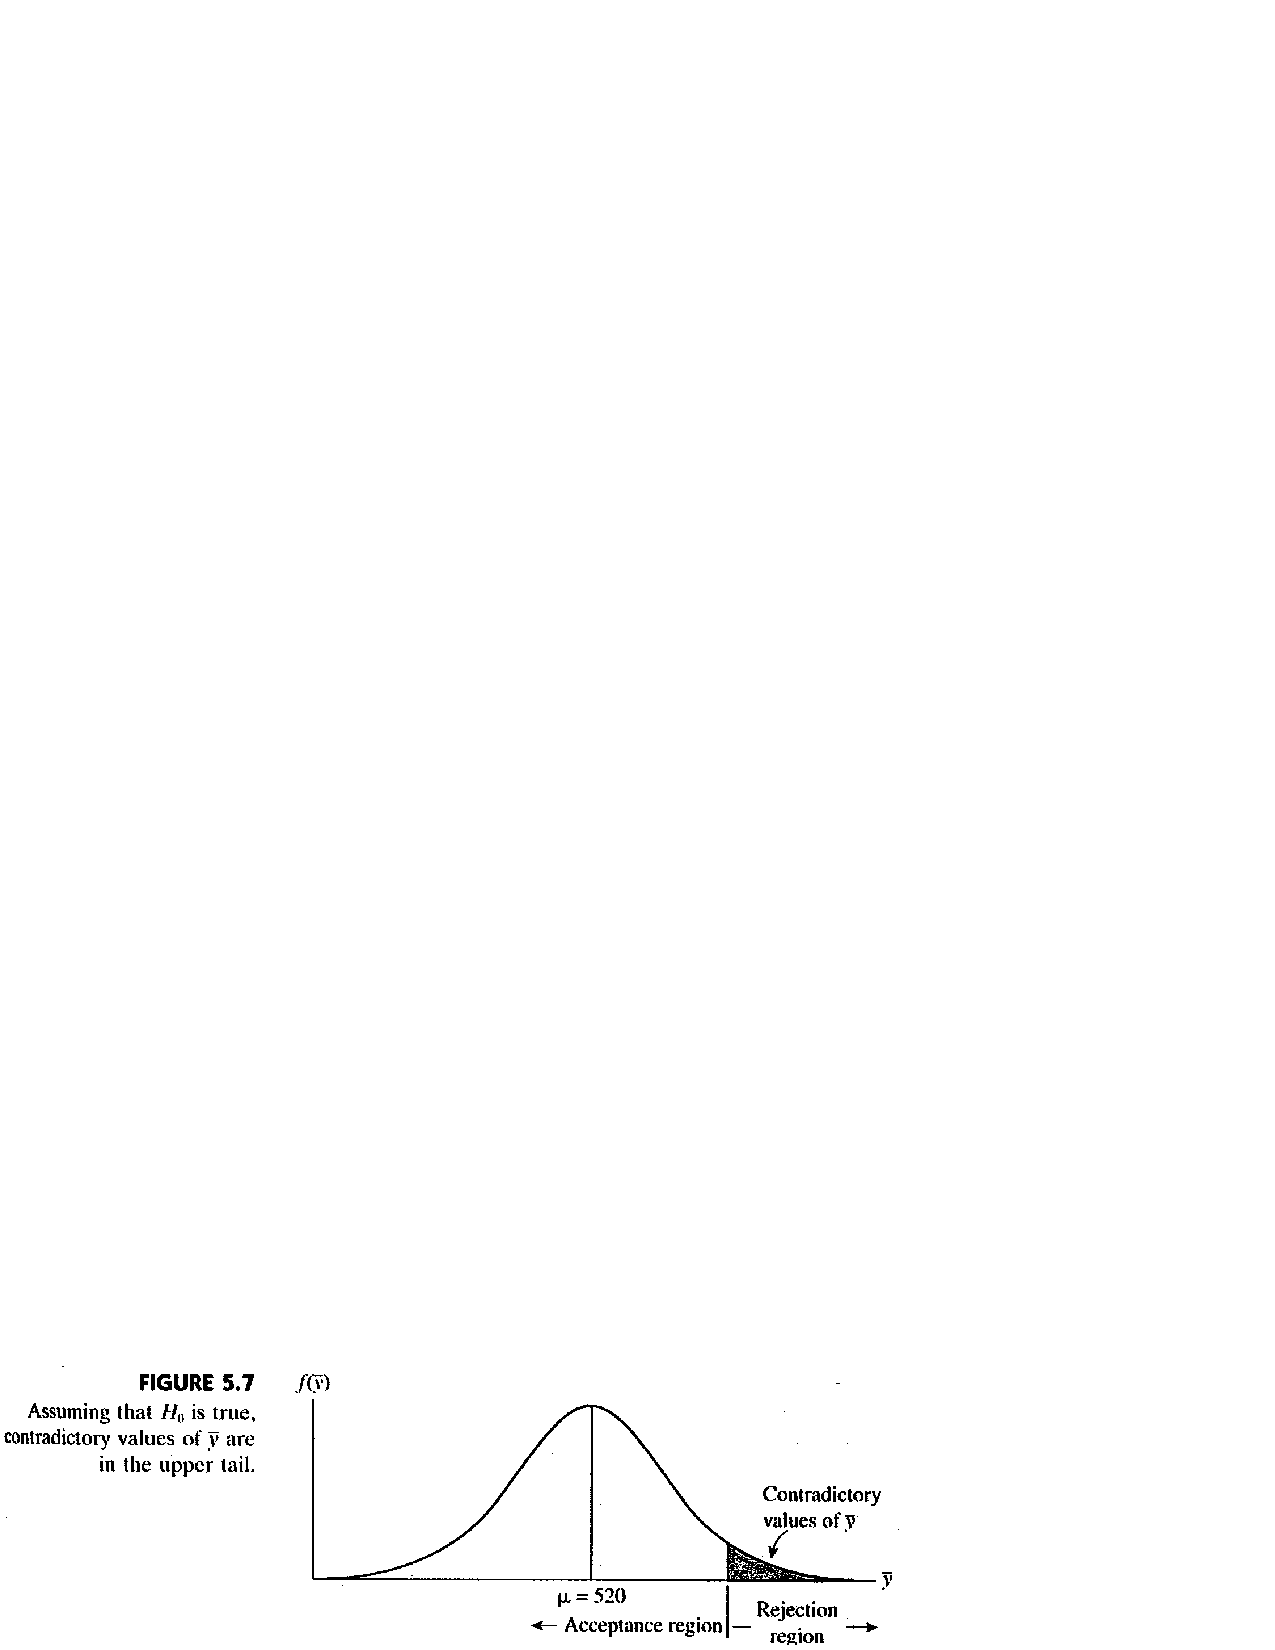
\includegraphics[trim={2cm 0cm 2cm 20cm},clip,scale=0.5]{fig57.pdf}
\end{center}
\end{frame}




%***********************************************************************
\begin{frame}
\frametitle{How to determine the rejection region}
\begin{itemize}
\item  By the CLT, $\bar{Y}$ is approximately a normal random variable.
\item  We will ignore
the approximation and assume $\bar{Y} \sim N(\mu, \frac{\sigma^2}{n})$. 
\item Then, for a given $\alpha$,
$$
  P \left( \frac{\bar{Y}-\mu}{\sigma/\sqrt{n}} > z_{\alpha} \right) = \alpha
$$
where $z_\alpha$ is the $1-\alpha$ quantile of the standard normal
distribution. 
\item So when $H_0: \mu \leq \mu_0$ is true ,
$$
  P \left( \frac{\bar{Y}-\mu_0}{\sigma/\sqrt{n}} > z_{\alpha} \right) \leq \alpha
$$
\end{itemize}
\end{frame}


\begin{frame}
\frametitle{How to determine the rejection region - cont.}
\begin{itemize}
\item  That is, 
$P(\bar{Y} > \mu_0 + z_\alpha \frac{\sigma}{\sqrt{n}})\leq \alpha.$ 
This suggests that we reject  $H_0: \mu \leq \mu_0$
in favor of, say $H_a: \mu > \mu_0$ when
$$
\bar{y} > \mu_0 + z_\alpha \frac{\sigma}{\sqrt{n}}
$$
(i.e., $\bar{y}$ is \textcolor{magenta}{too much}  when $\bar{y}$ exceeds the number $\mu_0 +
 z_\alpha \frac{\sigma}{\sqrt{n}})$\\
\item All possible $\bar{y}$ values satisfying $\bar{y} > \mu_0 + z_\alpha
\frac{\sigma}{\sqrt{n}}$ constitute the \textcolor{magenta}{rejection} \textcolor{magenta}{region}. 

\item  Instead of comparing  $\bar{y}$ to $\mu_0 + z_\alpha
\frac{\sigma}{\sqrt{n}}$, it is easier to first calculate 
$$
  z_c=\frac{\bar{y}-\mu_0}{\sigma/\sqrt{n}} 
$$
\end{itemize}
\end{frame}


\begin{frame}
\frametitle{How to determine the rejection region - cont.}
\begin{itemize}
\item We see that comparing $\bar{y}$ to $ \mu_0 + z_\alpha \frac{\sigma}{\sqrt{n}}$ is the same as comparing $z_c$ to $z_\alpha$.

\item That is, we reject the null hypothesis if $z_c > z_\alpha$ whis is the same thing as doing so if
$\bar{y} > \mu_0 + z_\alpha \frac{\sigma}{\sqrt{n}}$

 \item This  quantity $z$ is called
the \textcolor{magenta}{test statistic} and it's value can be calculated using the data
and the value $\mu_0$ specified in the null hypothesis $H_0$.
\item The notation $z_c$  is used denote the ``computed value'' of the test statistic, that is when we plug in the observed value of $\bar{y}$ and obtain a numerical value for $z$.
\end{itemize}
\end{frame}


\begin{frame}
\frametitle{Type I Error}
\begin{itemize}
\item  The $\alpha$ corresponds to the probability that the null
hypothesis is rejected when actually it is true and is called
the probability of committing a \textcolor{magenta}{Type I error}. 
\item Since the experimenter selects the value of $\alpha$  used in the test
procedure, she is able to specify or \textcolor{magenta}{control} the Type I error
rate or ``how much'' of this type of error is permitted in the 
testing procedure.
\end{itemize}
\end{frame}


\begin{frame}
\frametitle{Example }
Suppose from  a sample of 36 1-acre plots, the yield of corn this
year was measured and $\bar{y}=573$ and $s=124$ calculated.
Can we conclude that the mean yield of corn for all farms exceeded
520 bushels/acre this year ? Here we are going to assume that 
$\sigma$ can be approximated by $s$. Use $\alpha=.025$\\[.1in]
\end{frame}

 
 
\begin{frame}
\frametitle{Solution to the Example} 
\textcolor{magenta}{Set-up five parts of the testing procedure:}
\begin{enumerate}
\item $  H_0: \mu \leq 520$
\item $ H_a: \mu > 520 $
\item T.S.:  $z  =  \frac{\bar{y}-\mu_0}{\sigma/\sqrt{n}}$ 
\item R.R: Reject $H_0:$ in favor of $H_a:$ if $z > z_{.025}$ \\
 i.e. the R.R. is $z>1.96$ since $z_{.025}=1.96$
\item Compute the observed value of the test statistic:\\
 $z_c =\frac{573-520}{124/{\sqrt{36}}}= 2.56$
\end{enumerate}
\end{frame}




\begin{frame}
\frametitle{Decision:}
Since  $z_c> 1.96$,  $z_c$ is in the R.R. Thus $H_0:\mu \leq 520$ is rejected in favor of the
research hypothesis $ H_a: \mu > 520 $. It is  concluded that the 
mean yield this year exceeds 520 bushels/acre.\\[.1in]
Note that the above test procedure is equivalent to determining that
the  observed value for $\bar{y}$ lies more than 1.96 standard
deviations above the mean $\mu_0=520$.
\end{frame}



\begin{frame}
\frametitle{Summary of Test Procedures - Assume $n$ large, and $\sigma$ known}
\textcolor{magenta}{Hypotheses:}\\[.1in]
\textcolor{red}{Case 1:} $H_0: \mu \leq \mu_0\ \mbox{vs.}\ H_a: \mu >\mu_0$ (\emph{right-tailed test})\\[.1in]
\textcolor{red}{Case 2:} $H_0: \mu \geq \mu_0\ \mbox{vs.}\ H_a: \mu <\mu_0$ (\emph{left-tailed test})\\[.1in]
\textcolor{red}{Case 3:} $H_0: \mu = \mu_0\ \mbox{vs.}\ H_a: \mu \not =\mu_0$ (\emph{two-tailed test})\\[.1in]
\textcolor{magenta}{T.S:} $z_c  =  \frac{\bar{y}-\mu_0}{\sigma/\sqrt{n}}$\\[.1in]
\textcolor{magenta}{R.R:} For Type I error probability of $\alpha$:\\[.1in]
\textcolor{red}{Case 1:} Reject $H_0:$ if $z \geq z_{\alpha}$\\[.1in]
\textcolor{red}{Case 2:} Reject $H_0:$ if $z \leq -z_{\alpha}$\\[.1in]
\textcolor{red}{Case 3:} Reject $H_0:$ if $|z| \geq  z_{\alpha/2}$
\end{frame}



\begin{frame}
\frametitle{Decision:} 
If the computed value of the test statistic, $z_c$, is in the R.R.,
then we will reject the null hypothesis $H_0:$ at the specified $\alpha$ value. Otherwise, we say we fail to reject $H_0:$ 
at the specified $\alpha$ value.\\[.1in]
\textcolor{blue}{Example } {\small A corporation maintains a large fleet of company cars for its
salespeople.  To check the average number of miles driven per
month per car, a random sample of $n = 40$ cars is examined.  The
mean and standard deviation for the sample are 2,752 miles and
350 miles, respectively.  Records for previous years indicate that
the average number of miles driven per car per month was 2,600.  Use
the sample data to test the research hypothesis that the current
mean $\mu$ differs from 2,600.  Set $\alpha$ = .05 and assume that
$\sigma$ can be replaced by $s$.}
\end{frame}



\begin{frame}
\frametitle{Solution} 
The null hypothesis  for this statistical
test is $H_0: \mu$ = 2,600 and the research hypothesis is 
$H_a: \mu \neq$ 2,600.  Using $\alpha$ = .05, the two-tailed
rejection region for this test is $|z|> z_{.025}$ or
$|z|> 1.96$ and is located as shown below.
\begin{center}
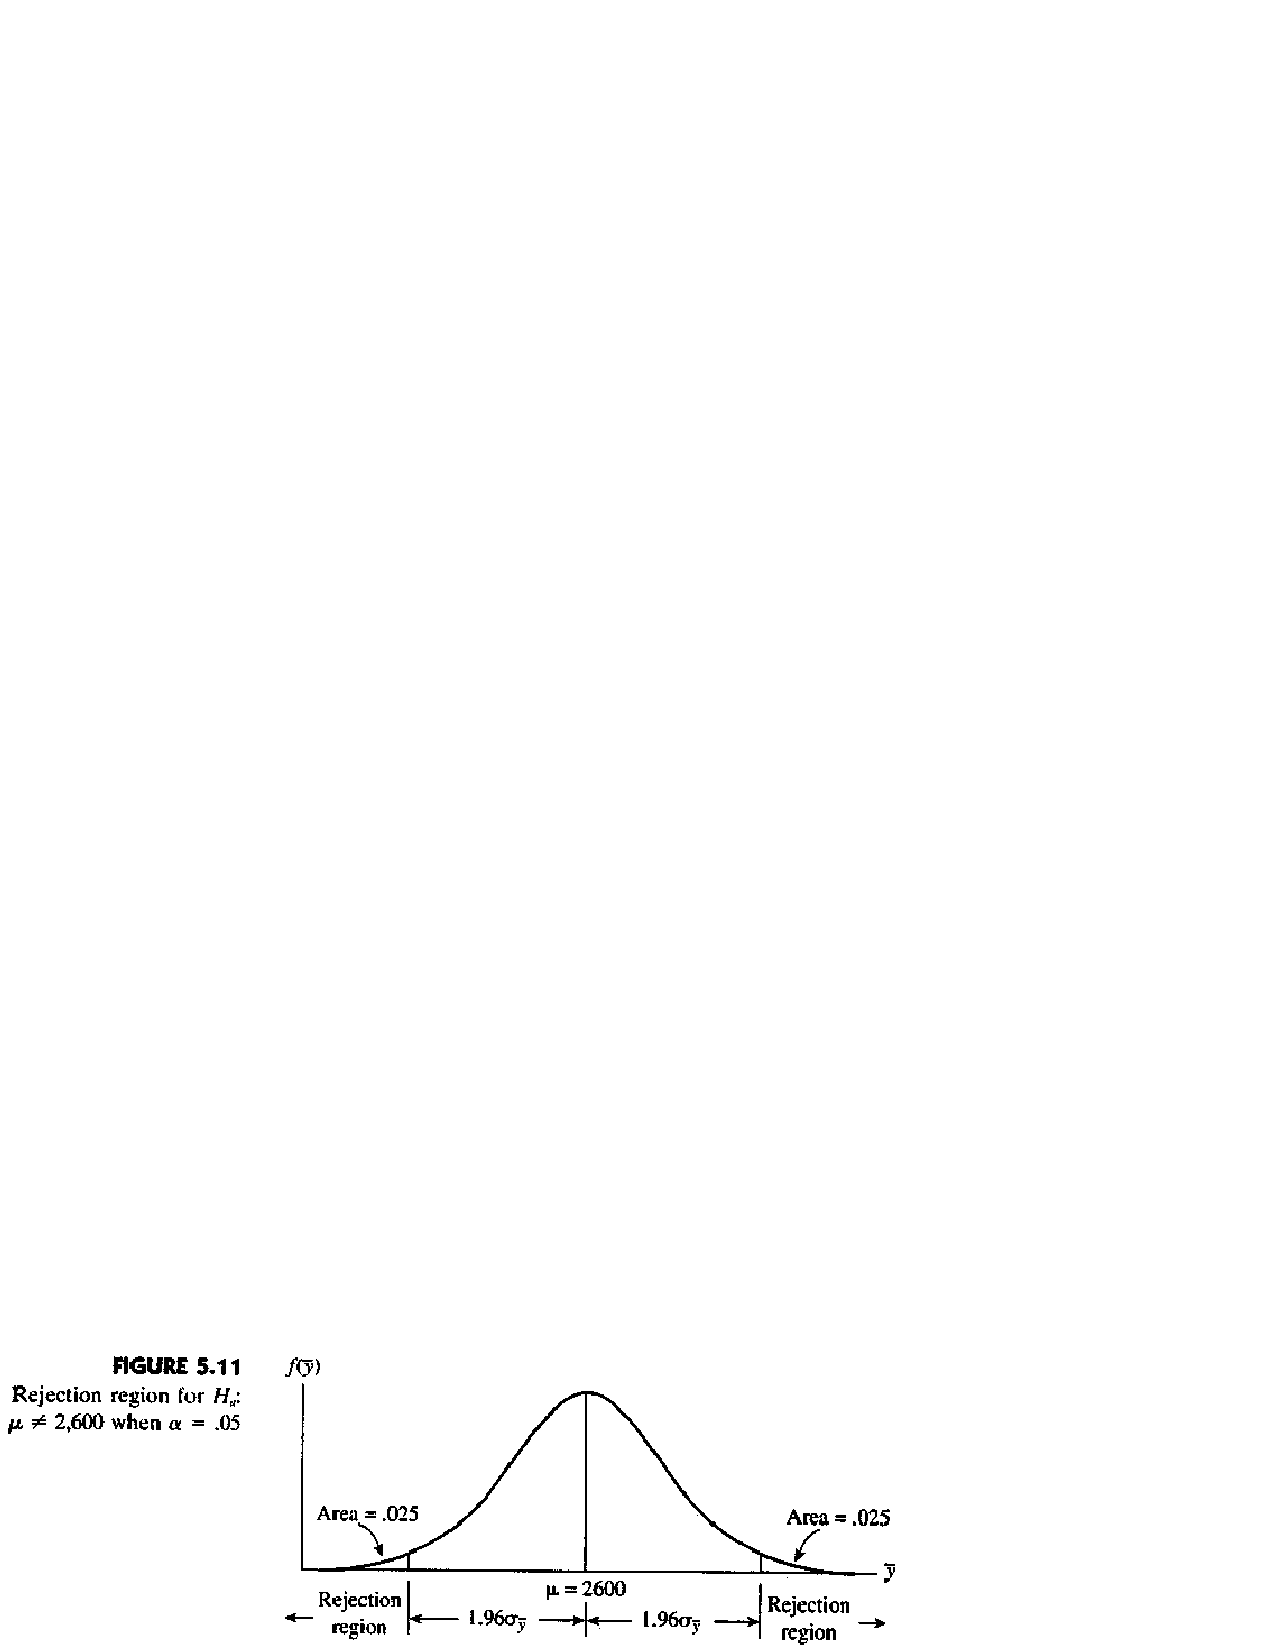
\includegraphics[trim={2cm 0cm 2cm 20cm},clip,scale=0.5]{fig511.pdf}
\end{center}
\end{frame}


\begin{frame}
\frametitle{Solution - cont.} 
To determine how many standard errors our test statistics
$\bar{y}$ lies away from $\mu$ = 2,600,  compute
$$
  z_c = \frac{\bar{y}-\mu_0}{\sigma/\sqrt{n}} =
  \frac{2,752 - 2,600}{350/\sqrt{40}} = 2.75 \, .
$$
Thus $|z_c|=2.75>1.96$ and therefore we reject   $H_0: \mu = 2,600 $
at $\alpha=.05$.
It follows that the observed value for $\bar{y}$ lies more than 
1.96 standard errors above the mean $\mu = 2,600 $, so we reject 
the null hypothesis in favor of the alternative $H_a: \mu \neq
2,600$. \\
 Since $\bar{y}>2,600$ we conclude that the mean number 
of miles driven is greater than $2,600$.
\end{frame}




\begin{frame}
\frametitle{Level of Significance or the p-value of a Statistical Test}
\begin{itemize}
\item   As an alternative to the formal test where one uses a rejection
region based on a specified the Type I error rate $\alpha$, 
many researchers compute and report the \textcolor{magenta}{level of 
significance} or  the  \textcolor{magenta}{p-value} for the test.  
\item This is the probability, when $H_0$ is true,  of observing a statistic as
extreme as the one actually observed.  Here ``extreme'' is  means ``large''
or ``small'' according to the alternative hypothesis $H_a$.
\end{itemize}
\end{frame}




\begin{frame}
\frametitle{Level of Significance or the p-value of a Statistical Test - cont.}
\begin{itemize}
\item Specifically, for a  given $\sigma^2$ and $\mu_0$ we find the p-value by:
\begin{enumerate}
\item[\textcolor{magenta}{1.}] First computing the test statistic,  $z_c$, 
       $$
         z_c = (\bar{y} - \mu_0)/(\sigma/\sqrt{n})
       $$
\item[\textcolor{magenta}{2.}]
      a) \ If $H_a: \mu > \mu_0$, then $p = P(Z > z_c$).\\
      b) \ If $H_a: \mu < \mu_0$, then $p = P(Z < z_c$).\\
      c) \ If $H_a: \mu \neq \mu_0$, then $p=2P(Z > |z_c|)$.
\end{enumerate}

\item A p-value smaller than the pre-specified $\alpha$ value is 
evidence in favor of rejecting $H_0$.
\end{itemize}
\end{frame}



\begin{frame}
\frametitle{Example:}
\begin{itemize}
\item In the earlier example we tested $H_0: \mu \leq 380\ \mbox{vs.}\ H_a: \mu > 380 $
Calculating the $z-$statistic,
$$
  z_c = \frac{\bar{y}-380}{\sigma/\sqrt{n}}= \frac{390-380}{35.2/\sqrt{50}} = 2.01 $$
  
\item The \textcolor{magenta}{level of significance}, or \textcolor{magenta}{p-value} for this test is
$$  p= P(Z > 2.01)= 1- P(Z < 2.01)= 0.0222$$
\item We \textcolor{magenta}{fail to reject} $H_0: \mu \leq 380$ at $\alpha=.01$ since p-value
is not less than $.01$
\end{itemize}
\end{frame}

%{\bf Interpreting p-values in SAS output}\\[.1in]
%\no The SAS output gives the p-values under columns
%labelled such as Prob$>|t|$ and is 
%{\tt the p-value calculated for the two-tailed
%test}. To convert this to a p-value to perform a one-tailed test: \\[.1in]
%\h \bul If  $H_a:\mu > \mu_0$ and computed statistic is positive\\[.1in]
%or\\
%\h \bul If  $H_a: \mu< \mu_0$ and computed statistic is negative\\[.3in]
%\h \h \h \fbox{take the p-value $ = ({\rm Reported\ value})/2$}\\[.1in]
%\h \bul If  $H_a: \mu > \mu_0 $ and computed statistic is negative\\[.1in]
%or\\
%\h \bul If  $H_a:  \mu< \mu_0$ and computed statistic is positive\\[.3in]
%\h \h \h  \fbox{take the p-value $ = 1- ({\rm Reported\ value})/2$}

\begin{frame}
\frametitle{{Inferences About \boldmath{$\mu$} when $\sigma$ is unknown}}
\begin{itemize}
\item For large sample sizes,  it follows from the CLT that $\bar{Y}$ is 
approximately Normally distributed i.e., $\bar{Y} \dot{\sim}
N(\mu,\frac{\sigma^2}{n})$. 
\item It follows that the random variable
$$
  T_{n-1} =\Big( \bar{Y} - \mu \Big) / \Big( S/\sqrt{n} \Big) 
$$
has approximately the \textcolor{magenta}{Student's $t$}
\textcolor{magenta}{distribution} with {$n-1$}
\textcolor{magenta}{degrees of freedom}. 

\item Here  $Y_1, Y_2, \ldots,Y_n$ are sampling random variables and $\bar{Y} =
\frac{1}{n} \displaystyle\sum_i Y_i$ is thus a random variable.
\end{itemize}
\end{frame}




\begin{frame}
\frametitle{{Inferences About \boldmath{$\mu$} when $\sigma$ is unknown - cont.}}
\begin{itemize}
\item The denominator of $T_{n-1}$ is the random variable
$$
  S = \sqrt{\frac{1}{n-1} \sum_{i=1}^n (Y_i - \bar{Y})^2}.
$$
\item If sampling from a Normal distribution, the sample mean  
$\bar{Y}$ has a Normal distribution (exactly) and therefore
$(\bar{Y}-\mu)/(S/\sqrt{n})$ will have a Student's $t$ distribution
(exactly),  regardless of sample size.
\end{itemize}
\end{frame}



\begin{frame}
\frametitle{}
\begin{itemize}
\item Until now, we have assumed that $n$ is large and
$\sigma$ is known, or $n$ is large and  $n$ is large enough also to
use $s$ as an  approximation to $\sigma$.  
\item Since we used the CLT to derive confidence limits and tests of hypotheses, 
 the exact nature of the sampled population was not required to be specified.

\item Now we require that  the population distribution to be Normal. 
We don't need to know $\sigma$ or have a large sample, i.e. $n$ to be large.
\item In this situation, for any $n$, ($\bar{Y} - \mu)/(S/\sqrt{n})$
will have a Student's t-distribution with d.f.$= n-1.$

\item Using this fact we can obtain confidence intervals and 
conduct tests of hypotheses even though $\sigma$ is unknown.  

\item Note the difference between $Z$ and $T_{n-1}$
is that the parameter $\sigma$ is in the denominator of $Z$.
\item That is, the point estimator of $\sigma$, $S$ is in the denominator of
$T_{n-1}$.
\end{itemize}
\end{frame}


\begin{frame}
\frametitle{Properties of the Student's \boldmath{$t$} distribution}
\begin{itemize}
\item There are many t-distributions each specified by a 
 single parameter called \textcolor{magenta}{degrees of freedom ($df$)}.
\item Like the standard normal population, the distribution
 is \textcolor{magenta}{symmetric} about 0 and has mean equal to 0.
\item The t-distribution has variance $df/(df-1)$, and hence is more
variable than the standard normal distribution which has variance
equal to 1. 
\item We say that the t-distribution has \textcolor{magenta}{heavier tails} than the 
standard normal distribution.
\item As the degrees of freedom $df$ increases, the t-distribution 
 approaches that of the standard normal distribution.
\item Thus as the sample size $n$ increases the distribution of the
 $T_{n-1}$ random variable approaches the standard normal distribution. 
\end{itemize}
\end{frame}



\begin{frame}
\frametitle{Properties of the Student's \boldmath{$t$} distribution cont.}
% insert figure 5.16 here
\begin{center}
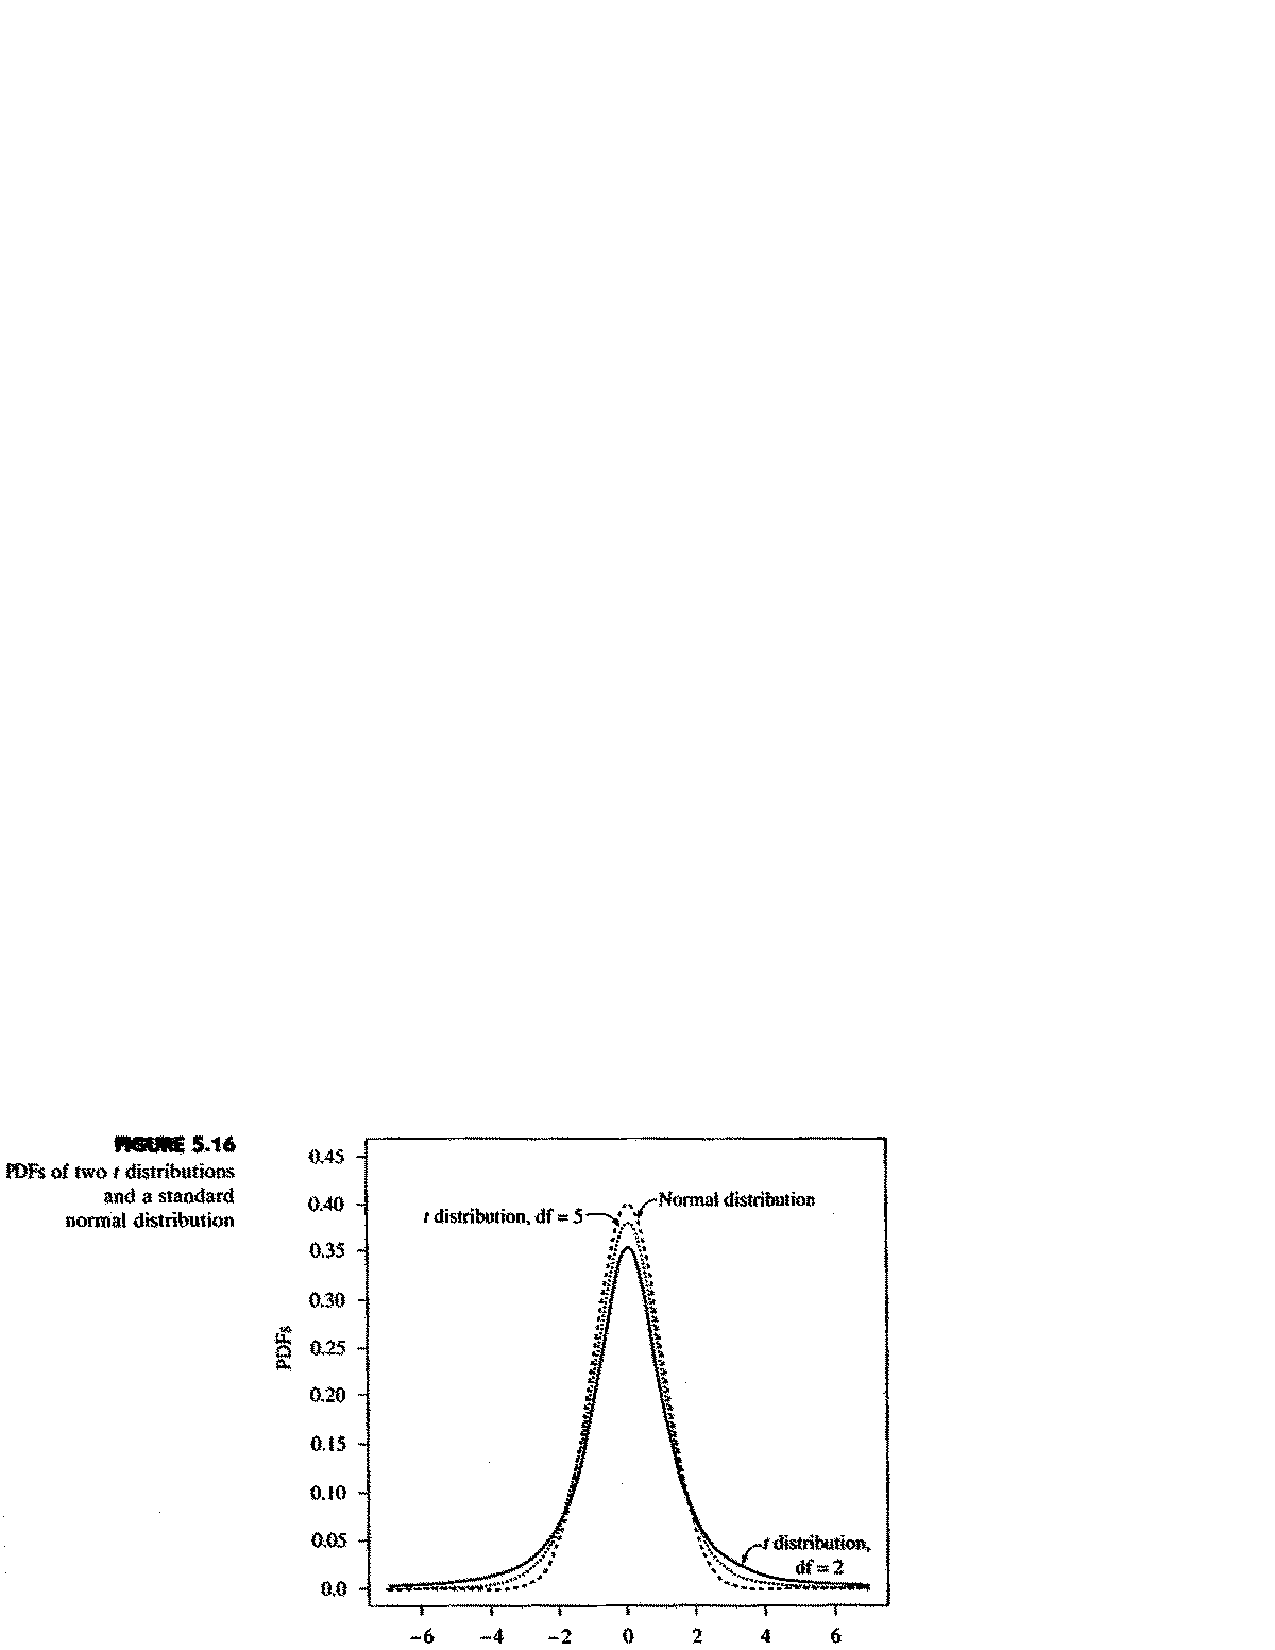
\includegraphics[trim={2cm 0cm 2cm 16cm},clip,scale=0.5]{fig516.pdf}
\end{center}
\end{frame}





\begin{frame}
\frametitle{}
The $t$ table gives quantiles 0.90, 0.95, 0.975, 0.99,
0.995, and 0.999 for $t$ distributions with selected \textit{df}.\\[.1in]
\textbf{Examples:  For $df = 10$}\\
$P(T_{10} > 1.372) = 0.10$\\
 $P(T_{10} < 1.372) = 0.90$\\
 $P(T_{10} > 1.812) = 0.05$\\[.1in]
If $\alpha$ = 0.05, then $t_\alpha$ satisfies $P(T_{10} > t_{.05}) = 0.05$
and from the t table , $t_{.05} = 1.812$. If $\alpha$ = 0.05, then $t_{\alpha/2} \, \equiv t_{0.025}= 2.228 $\\[.1in]
\textcolor{magenta}{Comparison of Normal and $t$ Quantiles}
\begin{center}
\begin{tabular}{lrrrrrrr}
\multicolumn{8}{c}{$t_\alpha$ with indicated df} \\[.1in] 
$\alpha$ & $z_\alpha$ & 10 & 20 & 30 & 40 & 60 & 240 \\ \hline
0.1  & 1.28 & 1.37 & 1.32 & 1.31 & 1.30 & 1.30 & 1.28 \\
0.05 & 1.65 & 1.81 & 1.72 & 1.70 & 1.68 & 1.67 & 1.65 \\
0.01 & 2.33 & 2.76 & 2.53 & 2.46 & 2.42 & 2.39 & 2.34 \\ \hline
\end{tabular}
\end{center}
\end{frame}




\begin{frame}
\frametitle{Confidence Interval for $\mu$ based on the t-distribution}
\begin{itemize}
\item Let the sample size be  $n$, and for $\alpha$ be a specified value, say, for e.g. $.05$.
\item  A $(1-\alpha)100\%$ confidence interval for $\mu$ is given by   
       $$ \left(\bar{y} - t_{\alpha/2} \, \frac{s}{\sqrt{n}}, \quad
        \bar{y} + t_{\alpha/2} \, \frac{s}{\sqrt{n}}\right)$$
\item This may also be written as  $ \left(\bar{y} - t_{\alpha/2} s_{\bar{y}}, \quad \bar{y} +
         t_{\alpha/2} s_{\bar{y}} \right)$ 
\item Here, $t_{\alpha/2}$ is the $1-\alpha/2$ percentile of the t-distribution with
$n-1$ degrees of freedom and $s_{\bar{y}}$ is the \textcolor{magenta}{standard error of the mean}.
\end{itemize}
\end{frame}



\begin{frame}
\frametitle{}
\begin{center}
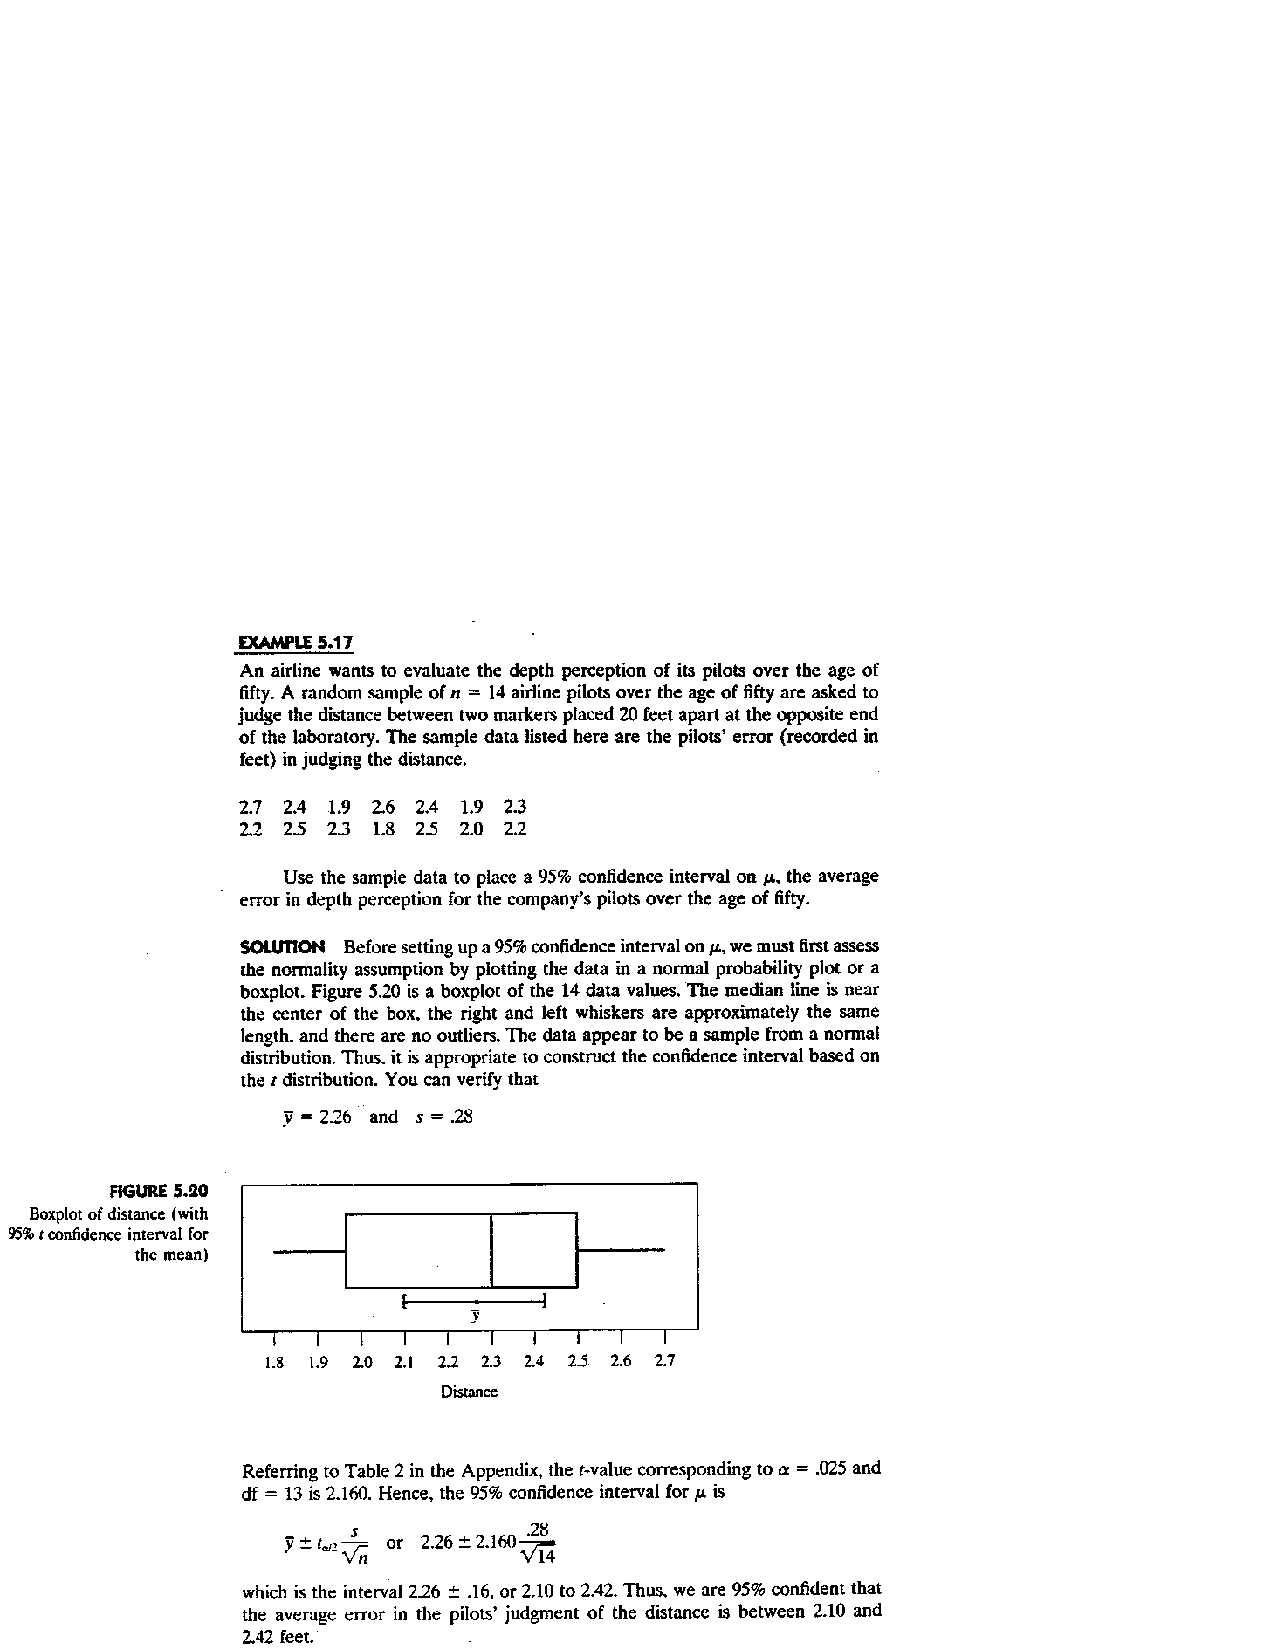
\includegraphics[trim={2cm 0cm 2cm 10cm},clip,scale=0.45]{ex517.pdf}
\end{center}
\end{frame}




\begin{frame}
\frametitle{Test Procedures based on the t-distribution:}
 \textcolor{magenta}{Hypotheses:}\\[.2in]
 \textcolor{red}{Case 1:}$H_0: \mu \leq \mu_0\ \mbox{vs.}\ H_a: \mu >\mu_0$ (right-tailed test)\\[.1in]
 \textcolor{red}{Case 2:} $H_0: \mu \geq \mu_0\ \mbox{vs.}\ H_a: \mu <\mu_0$ (left-tailed test)\\[.1in]
 \textcolor{red}{Case 3} $H_0: \mu = \mu_0\ \mbox{vs.}\ H_a: \mu \not =\mu_0$ (two-tailed test)\\[.1in]
 \textcolor{magenta}{T.S:} $t_c  =  \frac{\bar{y}-\mu_0}{s/\sqrt{n}}$\\[.2in]
\textcolor{magenta}{R.R:} For Type I error probability of $\alpha$:\\[.1in]
 \textcolor{red}{Case 1:} Reject $H_0:$ if $t \geq t_{\alpha,(n-1)}$\\[.1in]
 \textcolor{red}{Case 2:} Reject $H_0:$ if $t \leq -t_{\alpha,(n-1)}$\\[.1in]
 \textcolor{red}{Case 3:} Reject $H_0:$ if $|t| \geq t_{\alpha/2,(n-1)}$
\end{frame}





\begin{frame}
\frametitle{Test Procedures based on the t-distribution - cont.:}
\textcolor{magenta}{Level of Significance (p-value):}\\[.1in]
\textcolor{red}{Case 1:} $p = P(T_{n-1} > t_c$).\\
\textcolor{red}{Case 2:} $p = P(T_{n-1} < t_c$).\\
\textcolor{red}{Case 3:}  $p= 2P(T_{n-1} > |t_c|)$.\\[.3in]
\textcolor{magenta}{Exercise} \\[.1in]
A massive multistate outbreak of food-borne illness was attributed
to {\em Salmonella enteritidis}. Epidimiologists determined that the
source of the illness was ice cream. They sampled nine production
runsfrom the company that produced the ice cream to determine the
level of {\em Salmonella enteritidis}  in the ice cream.
\end{frame}



\begin{frame}
\frametitle{Exercise - cont.}
{\normalsize  These levels (MPN/g) are as follows\\[.1in]
 $.593\quad .142\quad .329\quad .691\quad .231\quad .793\quad .519\quad .392\quad .418$\\[.1in]
Use the data to determine whether the mean level of  {\em Salmonella
enteritidis}  in the ice cream is greater than .3 MPN/g with $\alpha=.01$}\\[.2in]
 \textcolor{magenta}{Solution:}\\[.1in]
Need to test $H_0: \mu \leq .3$ vs. $H_a: \mu > .3$ \\[.1in]
Because of the small sample size, we need to examine whether the 
data have been sampled from a normal distribution. To do this
a \textcolor{magenta}{normal probability plot} is a good tool.
\end{frame}



\begin{frame}
\frametitle{Exercise - cont.}
\begin{center}
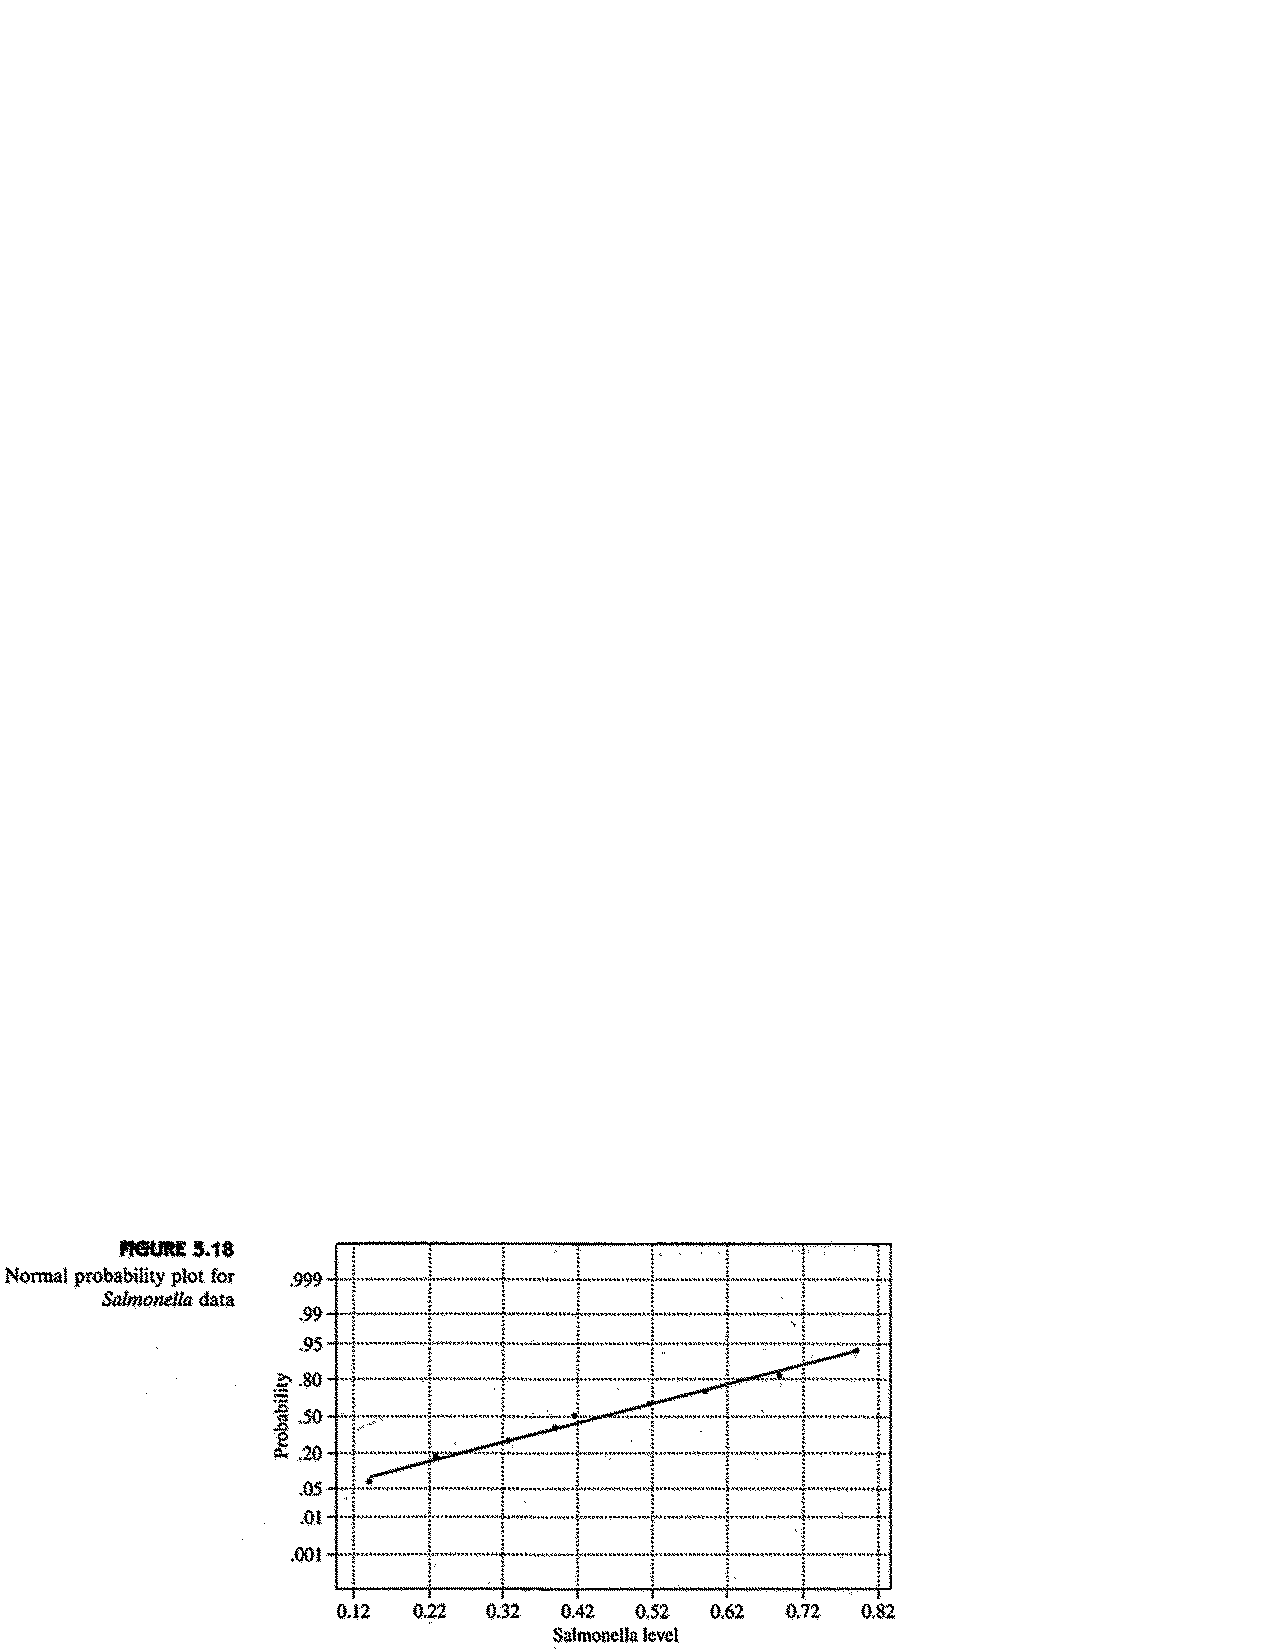
\includegraphics[trim={0cm 0cm 2cm 21cm},clip,scale=0.42]{fig518.pdf}
\end{center}
 From the data  $\bar{y}=.456$ and $s= .2128$ are computed, giving
$$ t_c=  \frac{\bar{y}-\mu_0}{s/\sqrt{n}}=\frac{.456-.3}{.2128/\sqrt{9}}=2.21$$
 Because for the one-tailed test we need $t_{\alpha,(n-1)}$;\\[.1in]
we look up  $t_{.01}$ with $df=9-1=8$. It is $ 2.896$\\[.1in]
Thus the rejection region is: $t>2.896$
\end{frame}



\begin{frame}
\frametitle{Exercise - cont.}
Since $t_c= 2.214$ does not exceed  $2.896$ it is not in the R.R.\\[.1in]
Thus, there is insufficient evidence in the data to reject $H_0$
i.e to say that the mean level of {\em Salmonella enteritidis}
exceeds the dangerous level of  .3 MPN/g.\\[.1in]
The \textcolor{magenta}{p-value} to be computed is $P(T_8>2.21)$\\[.1in] 
To calculate this exactly using the t-table is not possible
since it is tabulated for only a few values of $a$.\\[.1in]
However, we can bound the p-value by noting
that, for $(df=8)$, 2.21 lies between 1.86 and 2.306.\\[.1in] 
This gives \textcolor{magenta}{$.025<\mbox{p-value}<.05$} showing that the \textcolor{magenta}{p-value is not less than our $\alpha$ of $.01$}. Thus we fail to reject  $H_0$.
\end{frame}





\begin{frame}
\frametitle{OC Curve and the Power of a test}
The probabilities of the  four possible outcomes of a statistical test are:\\
\begin{tabular}{l|c|c} 
& \multicolumn{2}{c}{Null Hypothesis} \\ \cline{2-3}
Decision & True & False \\ \hline
Reject $H_0$ & \textcolor{red}{Type I Error} & Correct Decision \\
             & $\alpha$     & $1-\beta$ \\[.2in] \hline
Fail to reject $H_0$ & Correct Decision & \textcolor{red}{Type II Error} \\
             & $1-\alpha$       & $\beta$ \\
    \hline          
\end{tabular}
\begin{itemize}
\item The probabilities of Type I and II error are $\alpha$ and $\beta$,
respectively. 
\end{itemize}
\end{frame}



\begin{frame}
\frametitle{Type I Error and Type II Error}
\begin{itemize}
\item The experimenter can control only the Type I error probability. We do this by specifying an
$\alpha$ for an experiment (before the data values are measured).
\item When we are testing an hypothesis about  $\mu$ using  $\alpha$
for the test, the  value of \textcolor{magenta}{Type II error probability $\beta$} 
depends on the actual value $\mu$ which is not known.
\item This is because $\beta$ is the \textcolor{magenta}{probability of incorrectly failing to reject $H_0$ when $H_a$ is true}.
\item When $H_a$ is true, the actual value of $\mu$ may be any value under $H_a$, 
i.e, a value not specified under $H_0$. Since this value of $\mu$ is unknown,  
$\beta$  cannot be calculated.
\end{itemize}
\end{frame}



\begin{frame}
\frametitle{Type I Error and Type II Error}
\begin{itemize}
\item The implication of this is that when, based on a test, we
find that we cannot reject $H_0$, \emph{we will not say that we accept $H_0$}.
\item Because if we say  we accept $H_0$ and $\beta$ turns out to be large, then the 
probability is large that we will be committing a Type II error.
\item Thus the correct way to state the decision is to say, 
that \textcolor{magenta}{we fail to reject $H_0$}. 
\item In practice, $\beta$ probabilities for
several choices of $\mu$ (call them  $\beta(\mu)$) are calculated
and plotted in a graph called the \textcolor{magenta}{OC curve}. 
\item The OC curve can be used to read-off the \textcolor{magenta}{Type II error probability}
for a specified set of values sample size $n$ and $\alpha$.
\end{itemize}
\end{frame}


\begin{frame}
\frametitle{OC Curve}
\begin{center}
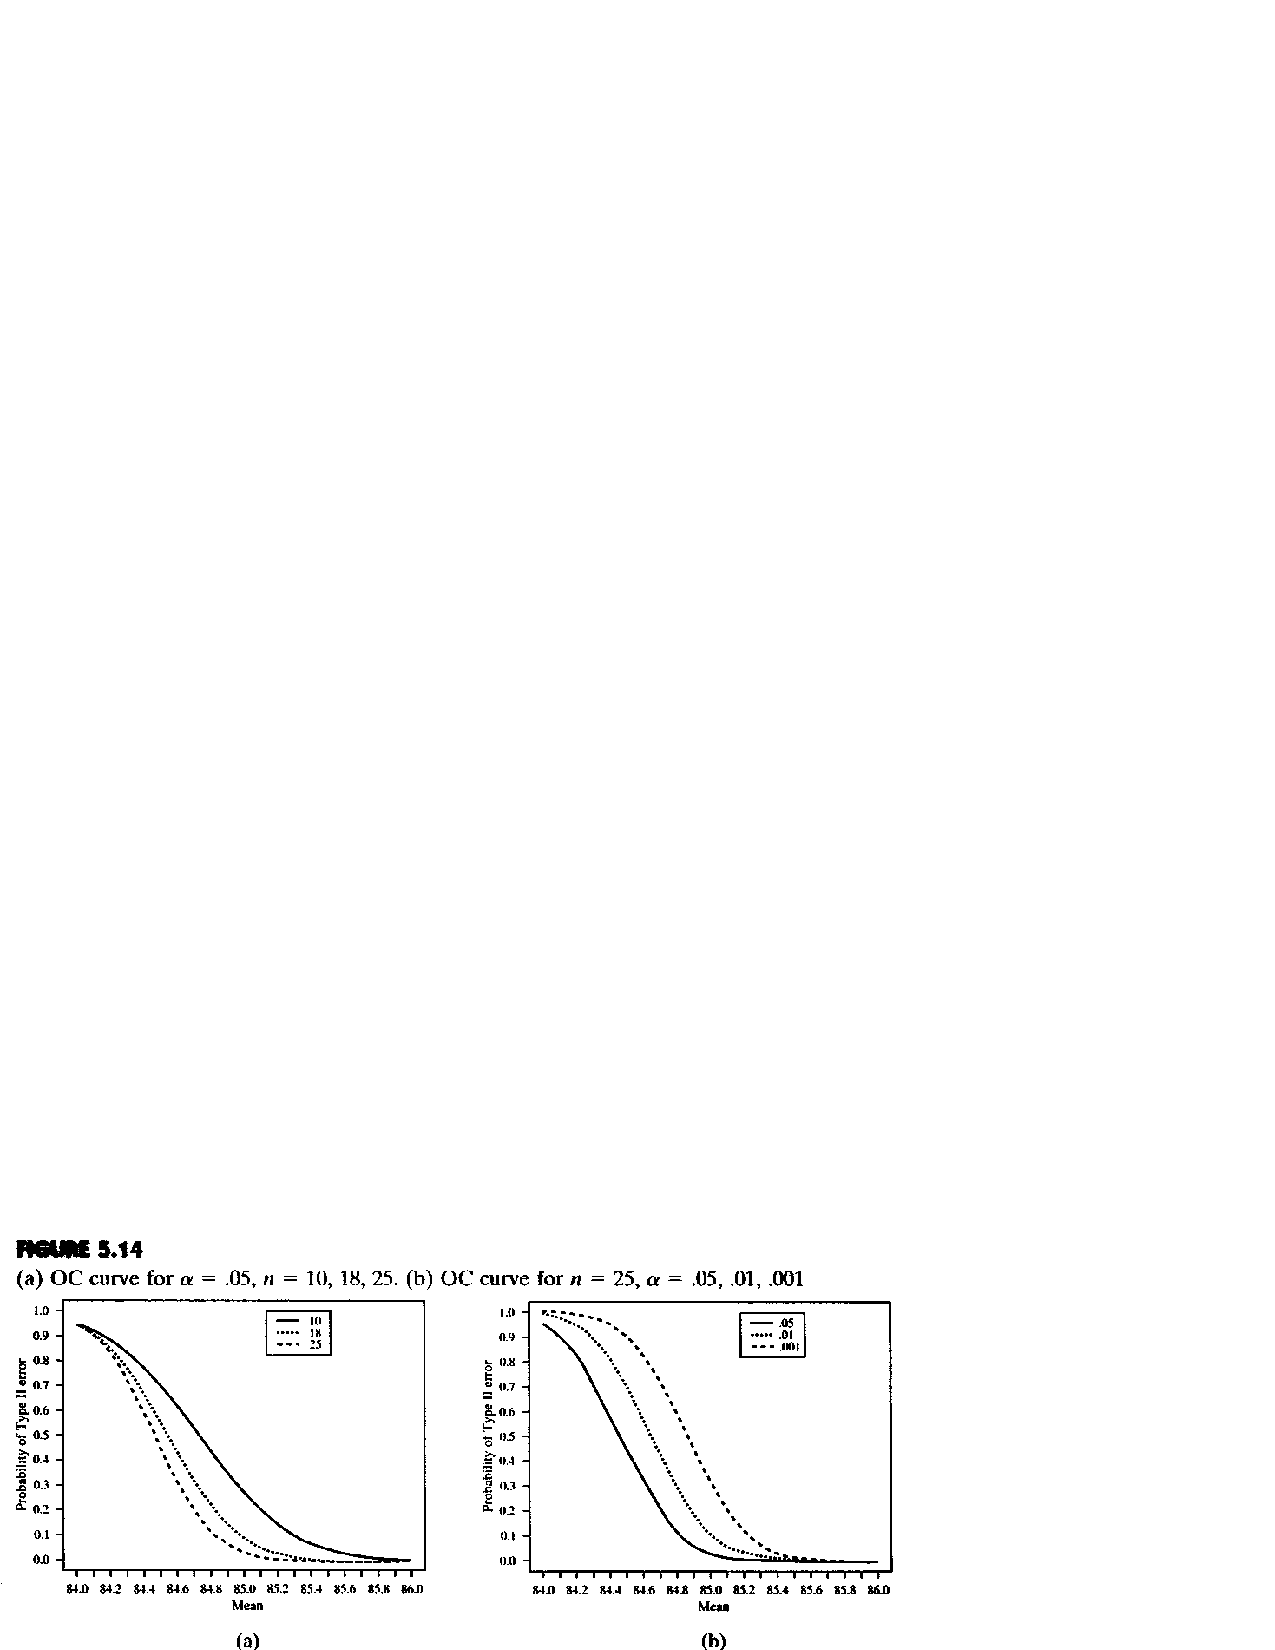
\includegraphics[trim={0cm 0cm 2cm 21cm},clip,scale=0.42]{fig514.pdf}
\end{center}
{\small The figure shows the OC curve for the test of 
$ H_0: \mu \leq 84, \quad H_a: \mu > 84$ for a population with 
$\sigma=1.4$. For example, for $\alpha=.05,\,n=10$, it can be 
seen that $\beta(84.8)\approx .4$ and that $\beta(84.8)$ decreases as 
sample size goes from 10 to 25. A conclusion that can be made
about this test from the OC curve is that Type II error probability 
would be $< .1$ for an actual $\mu > 84.8$ for $n=25$.}
\end{frame}


\begin{frame}
\frametitle{Power Curve}
\begin{itemize}
\item Another quantity that may be calculated for  a test procedure 
for a specified value of  $\mu$ is called the \textcolor{magenta}{Power
of the test} and is defined as $1-\beta(\mu)$.
\item The corresponding plot of power against a set of $\mu$ values 
is called the \textcolor{magenta}{power curve}. 
\end{itemize}
\end{frame}


\begin{frame}
\frametitle{Power of the Test}
\begin{itemize}
\item By definition, power of a test is the probability
of rejecting $H_0$ for a specified value of  $\mu$ under  $H_a$. 
\item In practice, tests are designed to have large power for some 
 $\mu$ values of interest so that they have small Type II error probabilities.
\item We can relate to this idea by thinking of a test as having very good power if it has  \textcolor{magenta}{a very good chance of detecting whether a change in $\mu$ has actually occured}.
 \item This is usually done by selecting a sample size $n$ to be used for
the experiment so that the desired power is achieved for a specified $\mu$ and $\alpha$.
\end{itemize}
\end{frame}

%\begin{center}
%\vspace*{-.5in}
%\epsfig{figure=graphs/ex_5.71.eps,height=7in,width=6.6in,clip=,angle=0,silent=}
%\end{center}


\begin{frame}
\frametitle{Using Type II Error Probability $\beta$ Curves}
\begin{itemize}
\item Consider the Salmonella example again.  We have $n=9,$ and $\alpha=.01$. Thus $df=8$ and we estimate $\sigma \approx .25$
\item We can compute the values of $d$ for several values of $\mu_a$. Then we'll read $\beta$ for those values of $d$ using the graph on next slide for the curves for $\alpha=.01$.
\item  As an example, for $\mu_a=.45$, $ d=\frac{|\mu_a-\mu_0|}{\sigma}=\frac{|.45-.3|}{.25}=.6$
\item Corresponding to $d=.6$ on the horizontal axis, using the curve for $df=8$ we see that $\beta(.45)=.79$, approx.
\item  Similarly, for $\mu_a=.45\ d=1.0$, and thus $\beta(.55)=.43$, approx. We can construct a table as shown (next slide).
\end{itemize}
\end{frame}



\begin{frame}
\frametitle{Using Type II Error Probability $\beta$ Curves}
\begin{center}
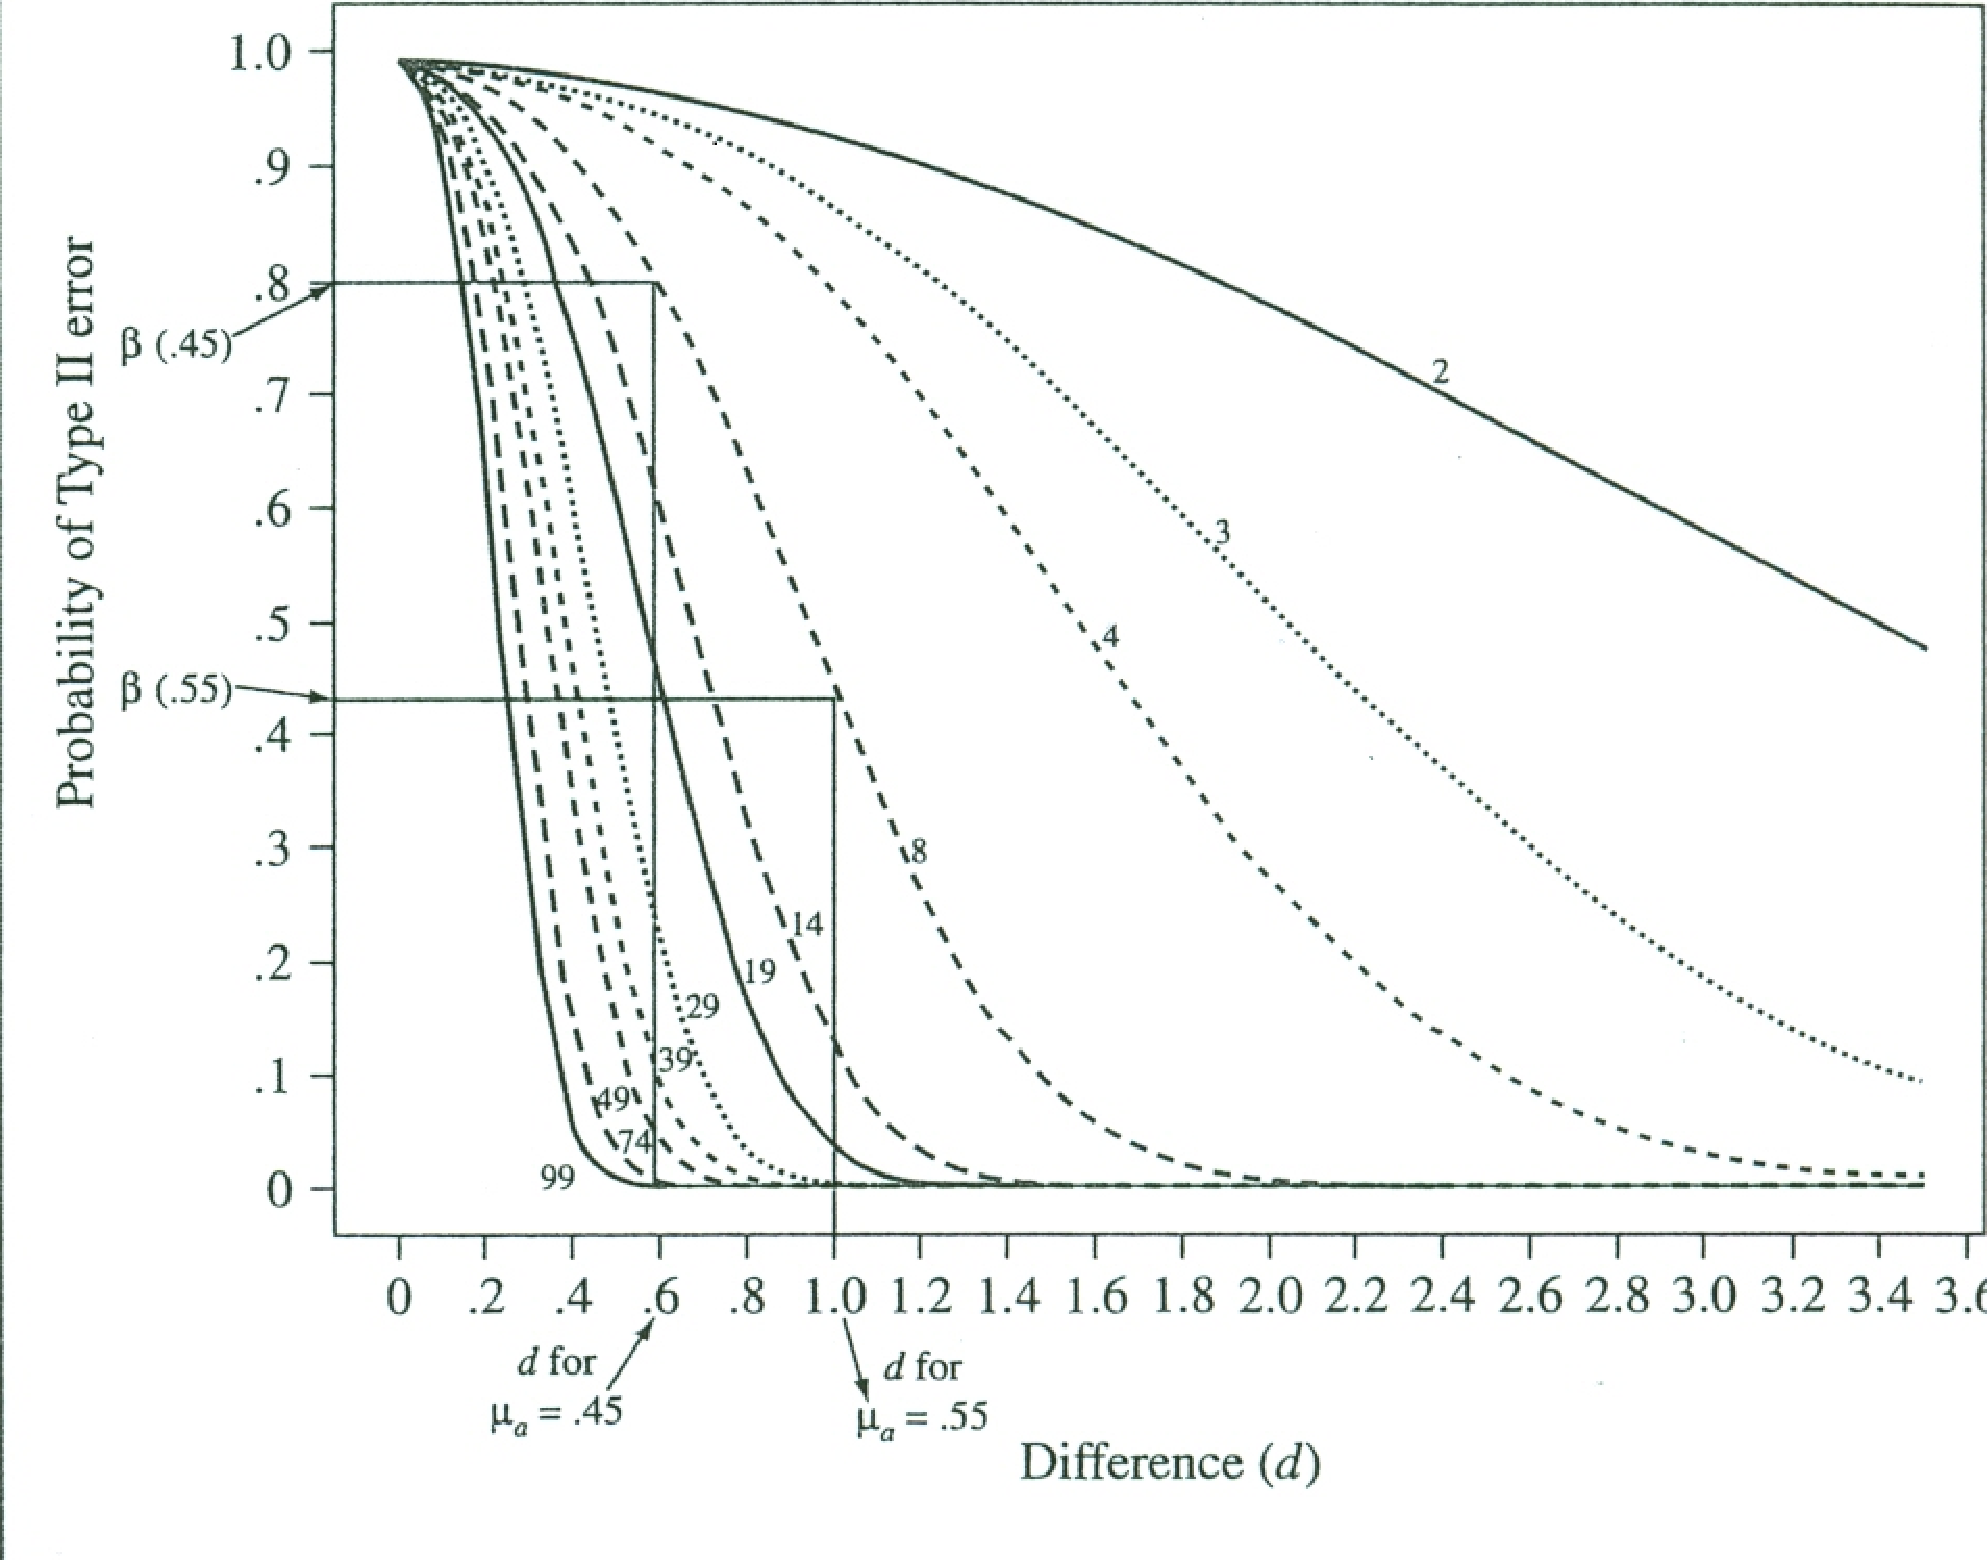
\includegraphics[scale=0.22]{fig517.pdf}\\[.1in]
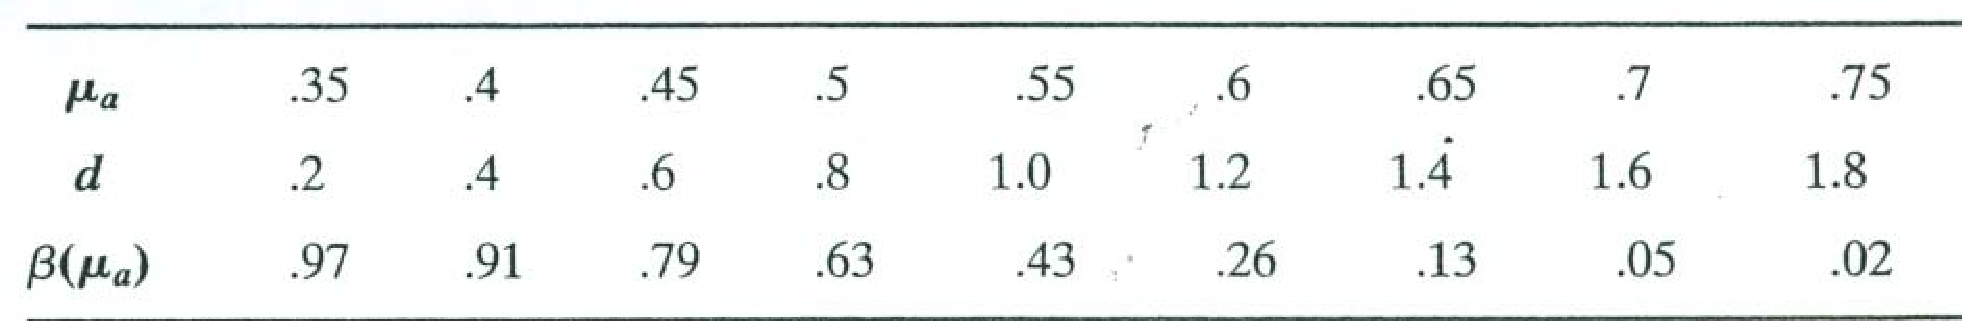
\includegraphics[scale=0.22]{table55.pdf}
\end{center}
\end{frame}




\begin{frame}
\frametitle{Departures from Normality}
\begin{itemize}
\item When $\bar{Y}$ is a Normal random variable, i.e., when sampling
from a Normal population with mean $\mu_0$,
$\frac{\bar{Y}-\mu_0}{S/\sqrt{n}}$ is a $T_{n-1}$ random variable.
\item This is a theoretical fact.  In practice, however, we never 
sample exactly from a Normal population, so
($\bar{Y}- \mu_0)/S/\sqrt{n}$ will be only approximately $T_{n-1}$.
\item How much effect can this have on C.I.'s and tests we construct?
\item For symmetrically distributed populations and
not too small $n$ there is little to worry about.
\item For highly skewed population distributions
the approximation can be terrible especially for small $n$.
\end{itemize}
\end{frame}




\begin{frame}
\frametitle{}
%insert table 5.6 here
\begin{center}
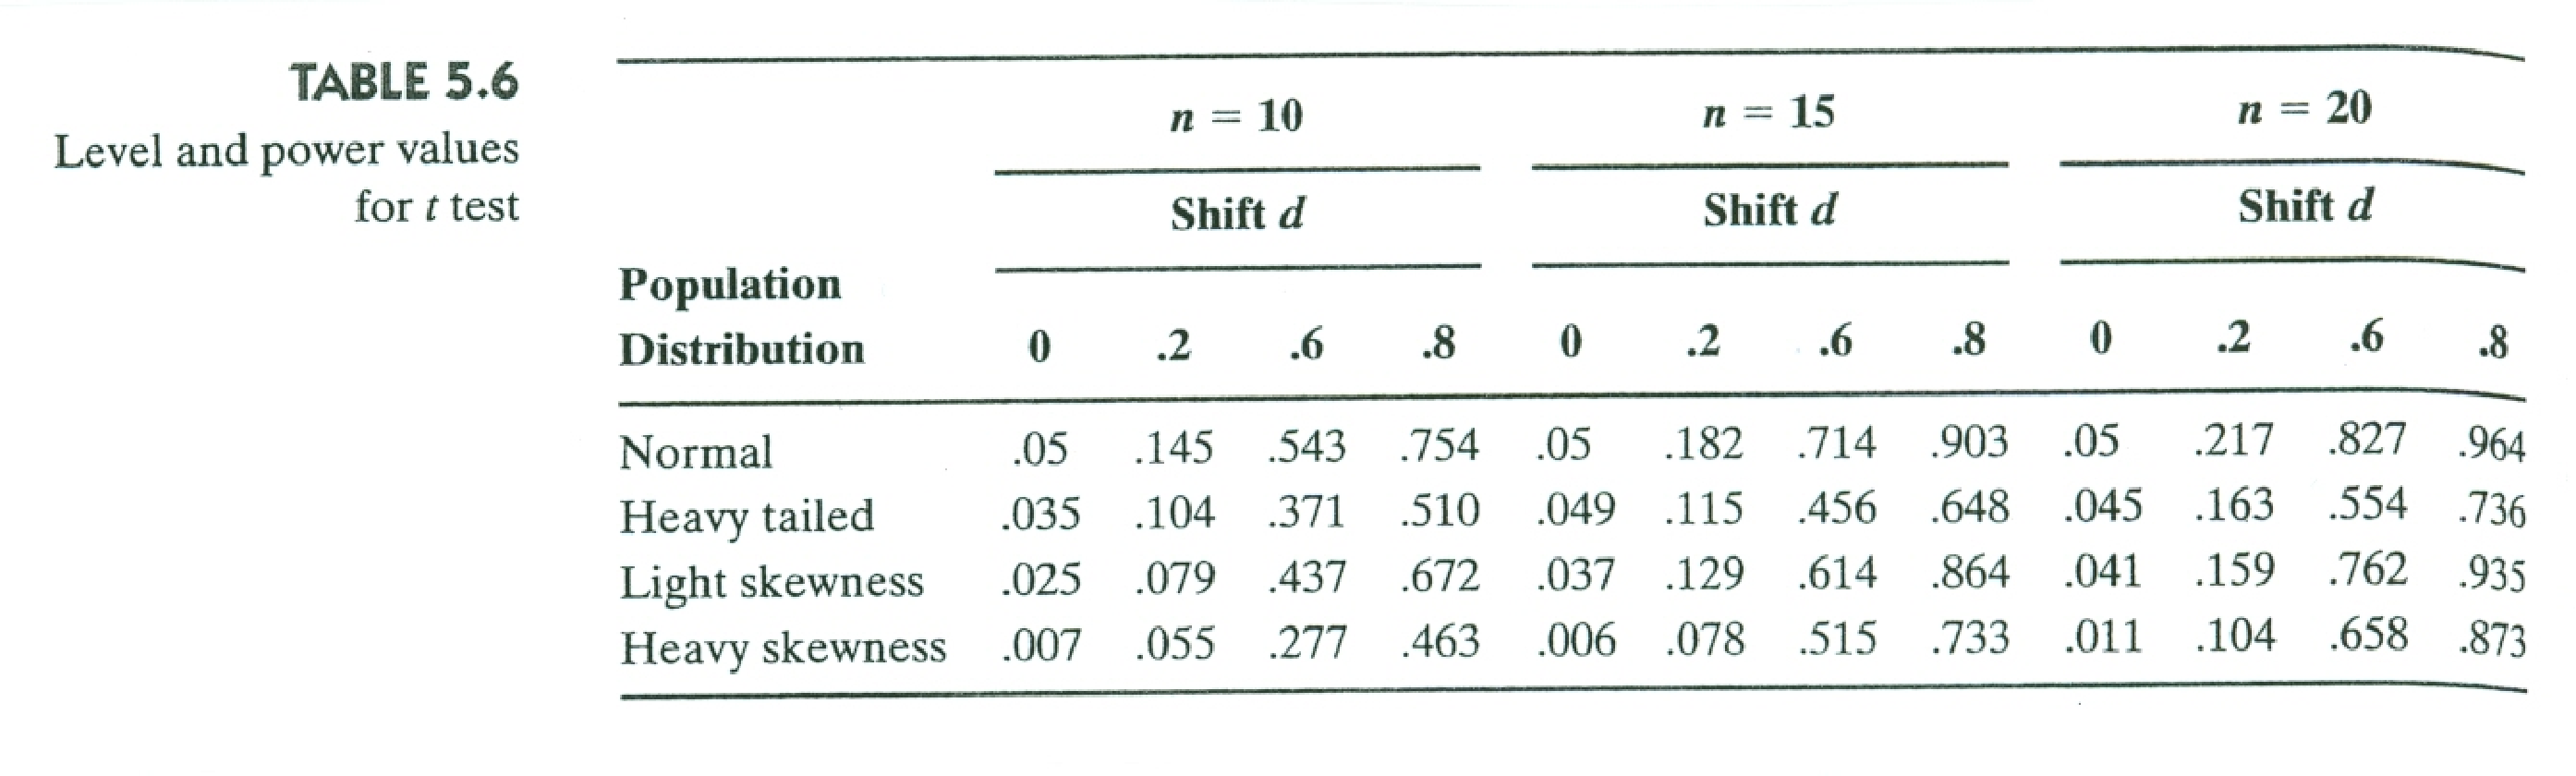
\includegraphics[scale=0.22]{table56.pdf}
\end{center}
\begin{itemize}
\item {\small It is recommended that one look at a boxplot, Normal plot, and/or
other graphics to see whether severe skewness of the
sampling population is indicated.  If not,
proceed to use the $t$-distribution.  If yes, one can use a
nonparametric procedure or use a transformation.  We will look 
at some of these later.}
\end{itemize}
\end{frame}



%***********************************************************************
\begin{frame}
\frametitle{Using Confidence  Intervals to Test Hypotheses}
\begin{itemize}
\item We can always look at a (1-$\alpha$)100\% confidence interval
and see what the result of a test would be if we carry out the
test. 
\item For example, consider the  (1-$\alpha$)100\% confidence
interval for $\mu$ 
  $$ \left(\bar{y} - t_{\alpha/2} \, \frac{s}{\sqrt{n}}, \quad
        \bar{y} + t_{\alpha/2} \, \frac{s}{\sqrt{n}}\right)$$
\item Suppose that  $\mu_0$ is \textcolor{blue}{not included} in the 
above confidence interval because
$$ \bar{y} - t_{\alpha/2} \, \frac{s}{\sqrt{n}}>\mu_0$$
\end{itemize}
\end{frame}



\begin{frame}
\frametitle{Using Confidence  Intervals to Test Hypotheses - cont.}
\begin{itemize}
\item By rearranging this we see that this is equivalent to $t_c$ being in the rejection
region, i.e.,\\
$$\frac{\bar{y}-\mu_0}{s/\sqrt{n}} > t_{\alpha/2,(n-1)}$$
\item Observe carefully that this is the same rejection region for
 the test of $H_0: \mu \leq  \mu_0$ vs. $H_a: \mu >
\mu_0$ at level  $\alpha/2$. 
\item That is, we will be rejecting $H_0$ \textcolor{magenta}{ at level  $\alpha/2$} if \\
$$\frac{\bar{y}-\mu_0}{s/\sqrt{n}} > t_{\alpha/2,(n-1)}$$
\item This is equivalent to saying that \textcolor{magenta}{if $\mu_0$ was not
included in a 100(1-$\alpha$)\% interval, then  $H_0$ 
will  be rejected if the test is  carried out at $\alpha/2$ level}.
\end{itemize}
\end{frame}


\begin{frame}
\frametitle{Using Confidence  Intervals to Test Hypotheses - cont.}
\begin{itemize}
\item  For \textcolor{magenta}{ a two-tailed test}, the confidence interval should be based on the same
$\alpha$ as the test to make this inference.
\end{itemize}
\textcolor{magenta}{\textbf{In summary,}}
\begin{itemize}
\item To test $H_0: \mu \leq \mu_0, \quad H_a: \mu > \mu_0$, at
level  $\alpha/2$, use a  100(1-$\alpha$)\% confidence interval.
\item To test $H_0: \mu \geq \mu_0, \quad H_a: \mu < \mu_0$, 
at level  $\alpha/2$, use a  100(1-$\alpha$)\% confidence interval.    
\item $H_0: \mu = \mu_0, \quad H_a: \mu \neq \mu_0$, 
at level  $\alpha$, use a  100(1-$\alpha$)\% confidence interval.   
\end{itemize}
\end{frame}
\end{document}

%***********************************************************************
\no \textbf{5.21}
A biologist wishes to estimate the effect of an antibiotic on the growth
of a particular bacterium by examining the mean amount of bacteria present per
plate of culture when a fixed amount of the antibiotic is applied.  Previous
experimentation with the antibiotic on this type of bacteria indicates that the
standard deviation of the amount of bacteria present is approximately $13\ cm^2$. 
Use this information to determine the number of observations (cultures that must
be developed and then tested) to estimate the mean amount of bacteria present,
using a $99\%$ confidence interval with a half-width of $3\ cm^2$.\\[.2in]
\h \h Take $\sigma =13,\quad E=3,\quad \alpha=.01 \quad z_{.005}=2.58$\\[.1in]
\h \h  Thus $$ n \geq \frac{(2.58)^2(13)^2}{(3)^2} = 124.99$$
\h \h  giving $ n=125$\\[.2in]
\no \textbf{5.31}
  The administrator of a nursing home would like to do a time-and-motion
study of staff time spent per day performing nonemergency tasks.  Prior to the
introduction of some efficiency measures, the average person-hours per day spent
on these tasks was $\mu = 16$.  The administrator wants to test whether the
efficiency measures have reduced the value of $\mu$.  How many days must be sampled
to test the proposed hypothesis if she wants a test having $\alpha=.05$ and the
probability of a Type II error of at most $.10$ when the actual
value of $\mu$ is 12 hours or less (at least a $25\%$ decrease from
prior to the efficiency measures being implemented)?  Assume $\sigma= 7.64$.\\[.2in]
\h \h  Test is $H_0: \mu \geq 16$ vs. $H_a: \mu <16 \quad at\ \alpha=0.05$\\[.1in]
\h \h  Want  $ \beta=0.10$, whenever $\mu\leq 12.$  Given  $\sigma= 7.64 $\\[.1in]
\h \h  Since $z_{.05}=1.645$ and $ z_{.10}=1.28,$ \\
$$ n= \frac{(7.64)^2(1.645+1.28)^2}{(12-16)^2}=31.2$$
\h \h giving $n=32$\\[.2in]
\no \textbf{5.49} \ Set up the rejection region based on $t$  for the
following conditions with $\alpha = .05$:\\[.1in]
\h \h  a. \ $H_a: \mu < \mu_0,\ \  n = 15$ \\
\h \h  b. \ $H_a: \mu \neq \mu_0,\ \  n = 23$\\
\h \h  c. \ $H_a: \mu > \mu_0,\ \  n = 6$\\[.1in]
\hspace*{1in}$\frac{\bar{Y}-\mu_0}{S/\sqrt{n}} \sim T_{n-1}$ \ when
$H_0$ is true.
\be
\item[a.] \ $t < -1.761$ is the rejection region for $\alpha$ = 0.05
     when $n=15,\ (df = 14)$.
\item[b.] \ $|t| > 2.074$ is the rejection region for
     $\alpha$ = 0.05, when  $n=23\ (df = 22)$.
\item[c.] \ $t > 2.015$ is the rejection region for
     $\alpha$ = 0.05,  when $n=6\ (df = 5)$.
\ee
\newpage
\no \textbf{5.51} \ The sample data for a $t$-test of $H_0: \mu \leq 15$
and $H_a: \mu > 15$ are $\bar{y} = 16.2$, $s = 3.1$, and
$n = 18$.  Use $\alpha$ = .05 to draw your conclusions.\\[.1in]
\hspace*{1in} $H_0: \mu \leq 15 \quad \mbox{vs.} \quad H_a: \mu > 15$\\[.1in]
Test statistic is: $t=\frac{\bar{y}-\mu_0}{s/\sqrt{n}}$.
For $\bar{y}  = 16.2,\ s = 3.1,\ n = 18$\\[.1in]
\hspace*{1in} $t_c = \frac{16.2 - 15}{3.1/\sqrt{18}} = 1.64$ \\[.1in]
\hspace*{1in} $t_{\alpha,df} \equiv t_{.05,17} = 1.740$ \\[.1in]
\hspace*{1in} R.R: $t> 1.74 $ \\[.1in]
Since $t_c = 1.64 < 1.74$, the computed t-statistic does not fall in the R.R.
Thus we fail to reject $H_0$ at $\alpha=0.05$\\[.2in]
\no Compute the $p$-value, i.e., find $p=P(T_{17}>1.64)$\\[.1in]
By looking through the tabulated t-values in Table 2 for $df=17$, we find that
1.64 corresponds to a p-value between 0.05 and 0.1 \\[.1in]
Again, since p-value is not smaller than .05, we fail to reject $H_0$.\\[.1in] 
\no \textbf{5.58} \ A dealer in recycled paper places empty 
trailers at various sites; these are gradually filled by
individuals who bring in old newspapers and the like.  The
trailers are picked up (and replaced by empties) on
several schedules.  One such schedule involves pickup every
second week.  This schedule is desirable if the average
amount of recycled paper is more than 1,600 cubic feet
per 2-week period.  The dealer's records for 18 2-week
periods show the following volumes (in cubic feet) at a
particular site:\\
{\small \begin{tabular}{rrrrrrrrr}
1,660 & 1,820 & 1,590 & 1,400 & 1,730 & 1,680 & 1,750 & 1,720 &
1,900 \\[.2in]
1,570 & 1,700 & 1,900 & 1,800 & 1,770 & 2,010 & 1,580 & 1,620 &
1,690 \\[.1in]
\end{tabular}}
\hspace*{.15in}{\small $(\bar{y} = 1718.3, s = 137.8)$}\\
\no a.) Assuming that the eighteen 2-week periods are fairly typical of
the volumes throughout the year, is there significant evidence that
the average volume $\mu$ is greater than 1,600 cubic feet ?\\[.1in]
\hspace*{.5in} $H_0: \mu \leq 1600 \quad H_a: \mu > 1600$ \\[.2in]
\hspace*{.5in} $ \quad t_c =
          \frac{1718.3-1600}{137.8/\sqrt{18}} = 3.64$ \\[.2in]
\hspace*{.5in} $\quad \alpha = 0.10, \ t_{.10,17} = 1.33$ \\[.2in]
\hspace*{.5in} R.R.: $t>1.33$ \\[.2in]
\hspace*{.5in} $t_c > 1.33$ so reject $H_0$ at  $\alpha = .10$.\\[.2in]
Thus a pick-up schedule of every second week is supported by the data.\\[.2in]
\no c.) Compute the $p$-value for the test statistic.\\[.2in]
When $H_0$ is true $\frac{\bar{Y}-1600}{S/\sqrt{n}}$ is a $T_{17}$
random variable and we observed the value $t = 3.64$.  
Thus $p = P(T_{17} > 3.64)$ is our $p$-value.  
In this case $p$ is close to 0.001, say, $p < 0.002$.\\[.2in]
\no b.)Place a $95\%$ confidence interval on  $\mu$.\\ 
\hspace*{.5in} $\alpha = 0.05,\quad t_{\alpha/2,df} = t_{.025,17}=2.11$\\
\hspace*{.5in}   compute\ \ $ 1718.3\ \pm\ (2.11)\cdot(\frac{(137.8)}{\sqrt{18}})$\\
\hspace*{.5in} to obtain $(1649.8,\ 1786.8)$.\\[.1in]
\no \textbf{5.60} \ A federal regulatory agency is investigating an
advertised claim that a certain device can increase the gasoline
mileage of cars.  Ten such devices are purchased and installed in
 cars belonging to the agency.  Gasoline mileage for each
of thecars  is recorded both before and after
installation.\\
{\small \begin{tabular}{lrrrrrrrrrrrrr}\\ \hline
& \multicolumn{7}{c}{Car}\\ \cline{2-11}
& 1 & 2 & 3 & 4 & 5 & 6 & 7 & 8 & 9 & 10 & n & $\bar{x}$ & s\\ \hline
Before(mpg)& 19.1 & 29.9 & 17.6 & 20.2 & 23.5 & 26.8 & 21.7 & 25.7 &
19.5 & 28.2 & 10 & 23.22 & 4.25\\
After(mpg) & 25.8 & 23.7 & 28.7 & 25.4 & 32.8 & 19.2 & 29.6 & 22.3 &
25.7 & 20.1 & 10 & 25.33 & 4.25\\
Change(mpg) & 6.7 & -6.2 & 11.1 & 5.2 & 9.3 & -7.6 & 7.9  & -3.4  & 6.2  &
-8.1  &10 & 2.11 & 7.54 \\  \hline
\end{tabular}}

\no Place $90\%$ confidence intervals on the average mpg for both before
and after phases of the study. Interpret these intervals. Does it
appear that the device will significantly increase the average
mileage of cars ?\\

\no \textbf{5.61} Refer to Exercise 5.60.\\
a. \ \parbox[t]{6in}{The cars in the study appear to have grossly
different mileages before the devices were installed. Use the change
data to test whether there has been a significant gain in mileage
after the devices were installed. Use $\alpha=.05$.}\\[.1in]
b. \ \parbox[t]{6in}{Construct a $90\%$ confidence interval for the
mean change in the mileage. On the basis of this interval, can one
reject the hypothesis that the mean change is either zero or
negative. (Note
that the two-sided 90\% confidence interval corresponds to a 
one-tailed $\alpha=.05$ test.)
}
\be
\item[a.] Need to test $H_0: \mu \leq \mu_0 \equiv 0$ vs. $H_a: \mu> 0$
 where $\mu$ represents the mean increase in gas mileage for a population
 of cars equipped with the device.\\
\hspace*{.5in}  $\bar{y} = 2.11, \quad s = 7.54$ \\[.1in]
\hspace*{.5in}  Thus $t_c = \frac{2.11 - 0}{7.54/\sqrt{10}} =0.88 $ \\[.1in]
\hspace*{.5in}   $ \alpha = 0.05 \ \ t_{.05,9} = 1.833 $\\[.1in]
\hspace*{.5in}      R.R.: $t> 1.833$\\[.1in]
Since  $t_c = 0.88 < 1.943 $ we fail to Reject $H_0$ at \\[.1in]  
$ \alpha=0.05$,
leading to the conclusion that there has not been a significant gain
in mileage due to the device.
\item[b.] A $90\%$ confidence interval is needed, i.e. $\alpha = .10$\\[.1in]
\hspace*{.5in} The interval is: $ \bar{y}\ \pm\ t_{\alpha/2,\ df}\cdot
\frac{s}{\sqrt{n}}$\\[.1in]
\hspace*{.5in} Plug-in the above values:  $ 2.11\ \pm\
1.833\cdot \frac{7.54}{\sqrt{10}} $\\[.1in]
\hspace*{.5in} giving the interval $(-2.26,\ 6.48)$.\\[.1in]
 Since $\mu_0=0$ is included in this interval we fail
to reject at  $H_0$ at  $\alpha =0.05$


\ee
\newpage
\no \textbf{5.90} \ Over the past 5 years, the mean time for a warehouse
to fill a buyer's order has been 25 minutes.  Officials of the
company believe that the length of time has increased recently,
either due to a change in the work force or due to a change in
customer purchasing policies.  The processing time (in minutes)
was recorded for a random sample of 15 orders processed over
the past month.
\begin{center}
\begin{tabular}{rrrrrr}
28 & 25 & 27 & 31 & 10 &\\
26 & 30 & 15 & 55 & 12 & \\
24 & 32 & 28 & 42 & 38 &
\end{tabular}
\end{center}
Do the data present sufficient evidence to indicate that the
mean time to fill an order has increased?  Use $\alpha$ =
.1.\\ 
\newpage
\no \hspace*{.5in} $H_0: \mu \leq 25$ against $H_a: \mu > 25$ \\[.2in]
\hspace*{.5in} $\bar{y} = 28.2, \ s_{\bar{y}} = 2.954, n = 15$ \\[.2in]
\hspace*{.5in} $t = \frac{28.2 - 25}{2.954} = 1.08 \quad$ \\[.2in]
\hspace*{.5in} $df = 14 \quad \alpha =.1 \quad  t_{0.1,14} = 1.345$\\[.2in] 
\no  Estimate p-value to be $ > 0.1$ from Table 2 in the
textbook.\\[.1in]   
In either case we fail to reject $H_0$ using $\alpha = 0.1$ .  
The evidence does not support an increase
in mean time to fill an order.

\no \textbf{5.108} \ In a random sample of 40 hospitals from a list
of hospitals with over 100 semiprivate beds, a researcher
collected information on the proportion of persons whose bills
are covered by a group policy under a major medical insurance
carrier.  The sample proportions are given in the following
chart.
\begin{center}
{\small \begin{tabular}{rrrrrrrr}
.67 & .74 & .68 & .63 & .91 & .81 & .79 & .73\\
.82 & .93 & .92 & .59 & .90 & .75 & .76 & .88\\
.85 & .90 & .77 & .51 & .67 & .67 & .92 & .72\\
.69 & .73 & .71 & .76 & .84 & .74 & .54 & .79\\
.71 & .75 & .70 & .82 & .93 & .83 & .58 & .84
\end{tabular}}
\end{center}
Use the sample data to construct a 90\% confidence interval on
$\mu$, the average proportion of patients per hospital with
group medical insurance coverage.\\[.2in]
\h \h $\bar{y} = 0.762, \quad s = 0.1086$\\[.2in]
\h \h $n = 40, \quad \alpha = 0.10, \quad t_{0.05,39} \approx 1.684$ \\[.2in]
We must compute\\[.2in]
\h \h \h \h $\bar{y}\ \pm\ t_{\alpha/2,\ df}\cdot (\frac{s}{\sqrt{n}})$ \\[.2in]
\h \h \h \h $0.762\ \pm\ (1.684)\cdot (\frac{.1086}{\sqrt{40}})$ \\[.2in]
The 90\% confidence interval is\\[.2in]
\h \h \h \h $(0.733, 0.791)$

\no \textbf{5.120} \ Doctors have recommended that we try to keep our
caffeine intake at 200 mg or less per day.  With the following
chart, a sample of 35 office workers were asked to record their
caffeine intake for a 7-day period.
\begin{center}
\begin{tabular}{ll}
coffee (6 oz) & 100--150 mg \\
tea (6 oz)    & ~40--110 mg \\
cola (12 oz)  & ~30 mg \\
chocolate cake & ~20--30 mg \\
cocoa (6 oz)  & ~~5--20 mg \\
milk chocolate (1 oz) & ~~5--10 mg
\end{tabular}
\end{center}
After the 7-day period, the average daily intake was obtained for
each worker.  The sample mean and standard deviation of the daily
averages were 560 mg and 160 mg, respectively.  Use these data to
estimate $\mu$, the average daily intake, using a 90\% confidence
interval.

\no \textbf{5.121} \ Refer to Exercise 5.120.  How many additional
observations would be needed to estimate $\mu$ to within $\pm$ 10
mg with 90\% confidence?\\
\textbf{5.120} \ $\bar{y} = 560,\quad s = 160, \quad n = 35,\quad \alpha = 0.10$ \\[.1in]
\hspace*{.5in} $t_{0.05,34} \approx  1.690 $ \\[.1in]
\hspace*{.5in} Plugging these in $\bar{y}\ \pm\ t_{\alpha/2}\cdot(\frac  {s}{\sqrt{n}})$\\[.1in]
\hspace*{.5in}  $560\ \pm\ (1.690)\cdot\frac{(160)}{\sqrt{35}}$\\[.1in]
\hspace*{.5in} $(514.3,\ 605.7)$ is the $90\%$ confidence
interval for average daily intake of caffeine.\\[.2in]
\no \textbf{5.121} \ The formula is
  $$
  n \geq \frac{(z_{\alpha/2})^2s^2}{E^2}
  $$
where $E$ is the half-width of the desired interval.

\no In this case $E = 10$, $z_{.05}=1.645 \quad \sigma = 160$
$$
  n \geq \frac{(1.645)^2(160)^2}{10^2} = 692.7 \, .
$$
Use$ n = 693 $ so we need $693-35 = 658$ more workers in the sample.}
















